\documentclass[journal,twoside,web]{ieeecolor}
\usepackage{jsen}
\usepackage{cite}
\usepackage{amsmath,amssymb,amsfonts}
\usepackage{algorithmic}
\usepackage{graphicx}
\usepackage{textcomp}
\usepackage{wrapfig}
\usepackage{lipsum}
\usepackage{float}
\usepackage{soul}
\usepackage{amsmath}
\usepackage{accents}
\usepackage[T1]{fontenc}
\usepackage{stfloats}
\usepackage{xr}
\usepackage{afterpage}
\externaldocument{sensors_metal_supplement}

\def\BibTeX{{\rm B\kern-.05em{\sc i\kern-.025em b}\kern-.08em
    T\kern-.1667em\lower.7ex\hbox{E}\kern-.125emX}}
\markboth{\journalname, VOL. XX, NO. XX, XXXX 2024}
{Author \MakeLowercase{\textit{et al.}}: Preparation of Papers for IEEE TRANSACTIONS and JOURNALS (May 2024)}
\definecolor{abstractbg}{rgb}{0.89804,0.94510,0.83137}
\setlength{\fboxrule}{0pt}
\setlength{\fboxsep}{0pt}

\begin{document}
\title{Evaluation of Metallic Interference in Electromagnetic Tracker for Handheld Robotics}
\author{Poonnapa Chaichudchaval, Robert A. MacLachlan, \IEEEmembership{Member, IEEE}, and Cameron N. Riviere, \IEEEmembership{Member, IEEE}
\thanks{Manuscript received May 5, 2025. This work was supported in part by the U.S. National Institutes of Health (grant nos. R01EB024564 and R01EB000526)}
\thanks{P. Chaichudchaval is with Department of Biomedical Engineering, Carnegie Mellon University, Pittsburgh, PA 15213 USA (email: pchaichu@andrew.cmu.edu). }
\thanks{R. A. MacLachlan is with Robotics Institute, Carnegie Mellon University, Pittsburgh, PA 15213 USA (email: robmacl@cmu.edu). }
\thanks{C. N. Riviere is with Robotics Institute, Carnegie Mellon University, Pittsburgh, PA 15213 USA (corresponding author; email: criviere@andrew.cmu.edu).
}}

\IEEEtitleabstractindextext{%
\fcolorbox{abstractbg}{abstractbg}{%
\begin{minipage}{\textwidth}%
\begin{abstract}
Metallic interference is a major limitation in electromagnetic trackers (EMTs). We systematically examined interference across multiple variables using the In-Loop Electromagnetic Tracker (ILEMT) with dual-frequency capability (300\,Hz and 10\,kHz) and compared results with pulsed DC modulation. We tested six metals in rod, tube, and sheet forms at multiple positions and orientations. These metals were both ferromagnetic and non-ferromagnetic, with varying electrical conductivities. Interference was very similar between the pulse and 300\,Hz modulations, with the benefit or harm of these low frequency modulations varying from a 260$\times$ decrease in interference to a 5.5$\times$ increase. It was often true that interference for ferromagnetic metals increased at low frequency while non-ferromagnetic metals showed a decrease, but the strength of this effect varied widely with shape and orientation, nearly disappearing or even reversing with large sheets. To build intuition about metal interference processes we include a substantial overview of the relevant physics. The relationship between magnetic field deviation and tracking error is nonlinear, with pose solution algorithms creating complex error patterns not predicted by field change alone. Metal interference decreased with distance following an inverse power law with exponents ranging from -3 to -6, with ferromagnetic materials and sheet samples near the theoretical -6 exponent predicted by dipole models, while non-ferromagnetic rod and tube samples showed significantly lower exponents. Shape and orientation significantly affected interference, with 90$^{\circ}$ rotations generally reducing the error. These findings provide practical guidance for EMT users in minimizing interference and offer EMT developers insights into the limitations of simple interference models, highlighting the potential of dual-frequency approaches for adaptive interference compensation.
\end{abstract}

\begin{IEEEkeywords}
eddy current, electromagnetic tracker (EMTs), metallic interference, permeability, skin effect 
\end{IEEEkeywords}

\end{minipage}}}

\maketitle

\section{Introduction}
\IEEEPARstart{T}{here} are two main tracking technologies used in handheld surgical navigation: optical and electromagnetic trackers (EMTs) \cite{sorriento_optical_2020}. Optical tracking is more common in orthopedic surgery due to its low latency and high resolution. Examples include camera tracking in NAVIO and CORI robotic systems for joint implantation, which precisely monitors both the joint and handheld instrument to improve implantation success \cite{adamska_robotic-assisted_2023}. Another example is Micron, a handheld device for micro-scale stabilization that uses an optical tracker called the Apparatus to Sense Accuracy of Position (ASAP) \cite{maclachlan_high-speed_2009,maclachlan_micron_2012}. ASAP uses Position-Sensitive Detectors (PSDs) with LED light markers to achieve high resolution and minimal latency.

However, optical trackers have a major limitation: they fail when visual obstructions block line-of-sight \cite{sorriento_optical_2020}. Since EMTs track motion by detecting changes in magnetic fields between a sensor and a source \cite{raab_magnetic_1979}, their low frequency magnetic fields freely penetrate tissue and most non-metal materials. This is particularly useful in Minimally Invasive Surgery (MIS), where precise tracking of specialized small tools inserted into the body is necessary \cite{chmarra_systems_2007}.

Despite this advantage, EMTs are sensitive to metallic interference as shown in \cite{sorriento_optical_2020, nixon_effects_1998}. When metallic materials are present in the workspace, the near-field phenomena causes two types of distortions: eddy currents and permeability effects. Most EMTs use either AC or pulsed DC signals, each responding differently to metals. AC trackers mostly experience eddy current distortions, so some commercial EMTs reduce interference by using lower carrier frequencies or pulsed DC. However, these approaches do not eliminate all interference. For example, tracking ultrasound tools showed position errors of 5 cm with pulsed DC trackers and 11.9 cm with AC trackers \cite{hastenteufel_effect_2006}. Similarly to the tracking orthopedic implants, it showed errors of 5.26 cm even with pulsed DC trackers \cite{milne_accuracy_1996}.

In this study, we systematically examine metallic interference in electromagnetic trackers using realistic materials and configurations. We evaluate multiple modulation approaches: the dual frequencies of In-Loop Electromagnetic Tracker (ILEMT) \cite{maclachlan_electromagnetic_2016, maclachlan_toward_2017} (300\,Hz and 10\,kHz) and the pulsed DC approach of commercial trackers. By analyzing how different metals interact with these modulation methods across various positions, orientations, and shapes, we provide insights into the underlying physical mechanisms of interference. We hope that this detailed analysis will help to build physical intuition about the interference mechanisms that EMTs may see in practical applications. This will help EMT users to configure an EMT compatible workspace and also suggests directions in EMT design for reduced metal interference.

\section{Related Work}

Higher conductivity generally leads to greater interference across different metal materials, though steel samples showed opposite results due to combined effects of permeability and eddy current \cite{stevens_minimizing_2010, lascalza_effect_2003}. Measurements with pulsed DC trackers found that steel samples produced greater error than aluminum at sampling rates between 20-140\,Hz, though aluminum caused more distortion at the highest sampling rate of 140\,Hz, as higher sampling rates provide less time for eddy current decay \cite{lascalza_effect_2003}. This confirms that eddy current distortion affects both ferromagnetic and non-ferromagnetic metals, specifically identified as out-of-phase distortion when developing mathematical models for interference correction \cite{cavaliere_enhancing_2023}.

Beyond material properties, studies in orthopedic tracking applications revealed that larger size and mass significantly increase distortion, while greater distance between metals and tracker components reduces interference \cite{stevens_minimizing_2010}. 

\begin{figure}[!htbp]
\centerline{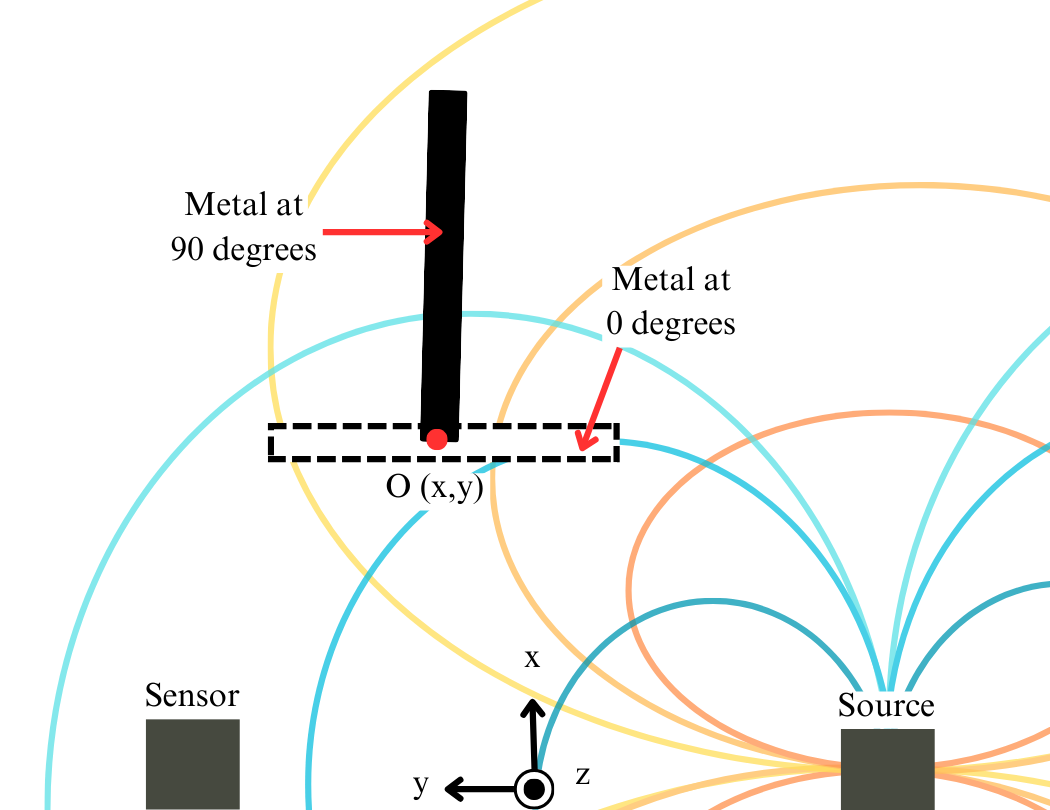
\includegraphics[width=\columnwidth]{chaic1.png}}
\caption{Visualization of the source magnetic fields that interact with interfering metal. For clarity, only the $x$ and $y$ fields are shown (the $z$ field would extend out of the page.) As the metal is rotated its alignment with the source fields changes, changing both the magnitude and direction of the fields measured at the sensor. The character of the field deviation also depends on the type of metal present. Reference point O indicates the measured position of the metal relative to the workspace origin.}
\label{magnetic_field}
\end{figure}

A dipole model predicting an inverse sixth power law for distance attenuation showed inconsistent results with large samples, while testing with sheet and cube samples demonstrated distortion increases proportionally to the sample width from the sensor perspective \cite{nixon_effects_1998}. Greatest interference occurs when metal is oriented parallel to the source-sensor plane, as metal orientation affects magnetic field blocking between source and sensor, as illustrated in Fig. \ref{magnetic_field} \cite{nixon_effects_1998}. Fully conductive closed loops create particularly strong interference by forming complete current paths within the magnetic field's projected area \cite{nixon_effects_1998}.

\section{EMT Operating Principles}
An EMT measures the position and orientation (pose) of a sensor relative to a magnetic source, providing six degrees of freedom (6 DOF) tracking. Since a single field measurement cannot fully determine the pose, EMTs utilize multiple source and sensor elements. In the systems we tested, the source generates three distinct magnetic fields, and the sensor measures these fields along three independent axes.

\subsection{Magnetic Coupling}
\label{subsec:coupling}
The magnetic interaction between source and sensor is quantified by a coupling matrix $\mathbf{C}$, where each element $\mathbf{C}_{jk}$ represents the coupling between source coil $j$ and sensor coil $k$ \cite{maclachlan_calibration_2025}. The sign of each coupling value indicates the direction of the magnetic field vector relative to the sensor coil orientation. This $3 \times 3$ coupling matrix contains all information needed to calculate the 6 DOF pose, but getting this pose requires inverting a magnetic model, which in general requires nonlinear optimization. 

When metallic objects are introduced into the tracking volume, they distort these magnetic fields, creating errors in the measured pose. While we are ultimately concerned with the pose error, measuring the field changes directly via the coupling matrix enables us to separate  the magnetic effects from the response of the pose solution algorithm. When a metallic object disturbs the source fields, the coupling matrix changes from an undisturbed state $\mathbf{C}$ to a disturbed state $\mathbf{C}'$. The coupling magnitude error is calculated as:
\begin{equation}
\text{Coupling Magnitude Error} = \frac{|\mathbf{C}' - \mathbf{C}|_2}{|\mathbf{C}|_2}
\end{equation}

Where $|\mathbf{A}|_2$ represents the matrix 2-norm. This normalization allows meaningful comparison of interference effects across different configurations, as it expresses the error relative to the undisturbed field strength.

\subsection{Tested EMTs}
\label{subsec:tested_emts}
EMTs require modulation of the source fields to allow the source axis signals to be separated from each other and from background fields. We tested two EMTs, ILEMT and trakSTAR. While these trackers have very different speed and resolution capabilities, they do represent the two main modulation principles used by EMTs: AC and pulse. 

\subsubsection{ILEMT}
The ILEMT open source EMT hardware is optimized for low noise and high measurement speed rather than cost \cite{maclachlan_electromagnetic_2016}. While a detailed discussion of ILEMT design and performance is outside the scope of this paper, typical performance with the tested source-sensor combinations is $<3\,\mu$m RMS position noise at 1500\,samples\,s$^{-1}$ (500\,Hz bandwidth) at a distance of 200 mm.

ILEMT employs frequency‑domain multiplexing: the three orthogonal source coils each transmit two continuous‑wave carriers---a low‑frequency tone (274\,Hz, 334\,Hz, 370\,Hz) and a high‑frequency tone (7.5\,kHz, 10.5\,kHz, 13.5\,kHz)---so all six tones are unique and can be demodulated concurrently. The high‑frequency set lies in the range commonly used by inductive AC trackers, giving good signal--to--noise ratio, wide measurement bandwidth, and sub‑millisecond latency for closed‑loop control. Field strength is kept identical at both bands, but the sensor signal is much weaker at low frequency, so the low‑band data are acquired at 12\,samples\,s$^{-1}$ with a 3\,Hz bandwidth to maintain noise performance. The low‑frequency measurements are less prone to eddy‑current interference than their high‑frequency counterparts, so combining the two bands in a Kalman filter yields fast dynamics together with reduced metal‑induced error, provided the interfering metal moves only slowly. For brevity, the remainder of the paper refers to the high‑frequency carriers as ``10\,kHz'' and the low‑frequency carriers as ``300\,Hz''.

\subsubsection{trakSTAR}
While ILEMT is a research prototype, the 3D Guidance trakSTAR (NDI Inc.) is a mature commercial EMT product aimed at medical applications. It typically operates at 80\,samples\,s$^{-1}$, with a specified resolution of $500\,\mu$m at 300 mm source-sensor distance. The position output is quantized at $110\,\mu$m increments, giving a hard limit to the minimum error that can be detected. 

 trakSTAR uses pulse modulation and a DC responding flux-gate sensor, which allows it to operate with a much lower modulation frequency than AC EMTs normally use. The implementation is in the time domain. The source creates a step change in the field, and then the sensor measurement is delayed to allow eddy currents to decay. The measurement is time domain multiplexed with each axis pulsed in turn. In trakSTAR, with 80\,samples\,s$^{-1}$ output rate, each axis has a 1.5 ms background measurement, then a 2.5 ms pulse. This gives an effective modulation frequency of 250\,Hz, but harmonics from the pulse modulation also affect the measurement. So the effective modulation frequency is similar to the ~300\,Hz low frequency modulations used by ILEMT.

\section{Metal Interference Theory}

\subsection{Magnetic Dipole Model}

The dipole is the simplest physical model for the electromagnetic tracker's source field and provides a foundation for understanding metal interference effects \cite{griffiths_introduction_1999}. A magnetic dipole is characterized by two parameters: location $\mathbf{l}$ and vector moment $\mathbf{m}$. When a sensor is located at position $\mathbf{p}$, the magnetic field $\mathbf{B}(\mathbf{p})$ is given by:
\begin{equation}
\mathbf{B}(\mathbf{p}) = \mu \frac{1}{|\mathbf{r}|^3} [3(\mathbf{m} \cdot \mathbf{\hat{r}})\mathbf{\hat{r}} - \mathbf{m}]
\label{eq:dipole_field}
\end{equation}

where $\mathbf{r} = \mathbf{p} - \mathbf{l}$, $\mathbf{\hat{r}} = \frac{\mathbf{r}}{|\mathbf{r}|}$, and $\mu$ is the permeability of the medium. This equation shows that the magnetic field vector depends not only on distance but also on the relative orientation between the moment vector and position vector.

The sensor performs a three-dimensional vector measurement of this magnetic field. This vector nature is crucial for understanding metal interference, as the interaction depends on the orientation of the metal relative to the field vectors.
\subsection{Nixon's Field Interference Model}
\label{nixon_model}
Building on this dipole model, we can derive the relationship between metal interference and tracker error. While the source creates vector fields, for analytical simplicity we will use Nixon's scalar potential model\cite{nixon_effects_1998}. We start with the relationship between potential field $v$ and distance $r$:
\begin{equation}
v \propto r^{-3}
\label{eq:field_distance}
\end{equation}

For position determination, this relationship is inverted to find distance from measured field:
\begin{equation}
r \propto v^{-1/3}
\label{eq:distance_field}
\end{equation}

When a small error $\Delta v$ occurs in the measurement, it creates a position error $\Delta r$. Taking the derivative of equation \eqref{eq:distance_field} and substituting from \eqref{eq:field_distance}, we find $\Delta r = \frac{dr}{dv}\Delta v = -\frac{r^4}{3}\Delta v\propto r^4\Delta v$. This shows that position error sensitivity increases with the fourth power of source-to-sensor distance.

\begin{figure}[!htbp]
\centerline{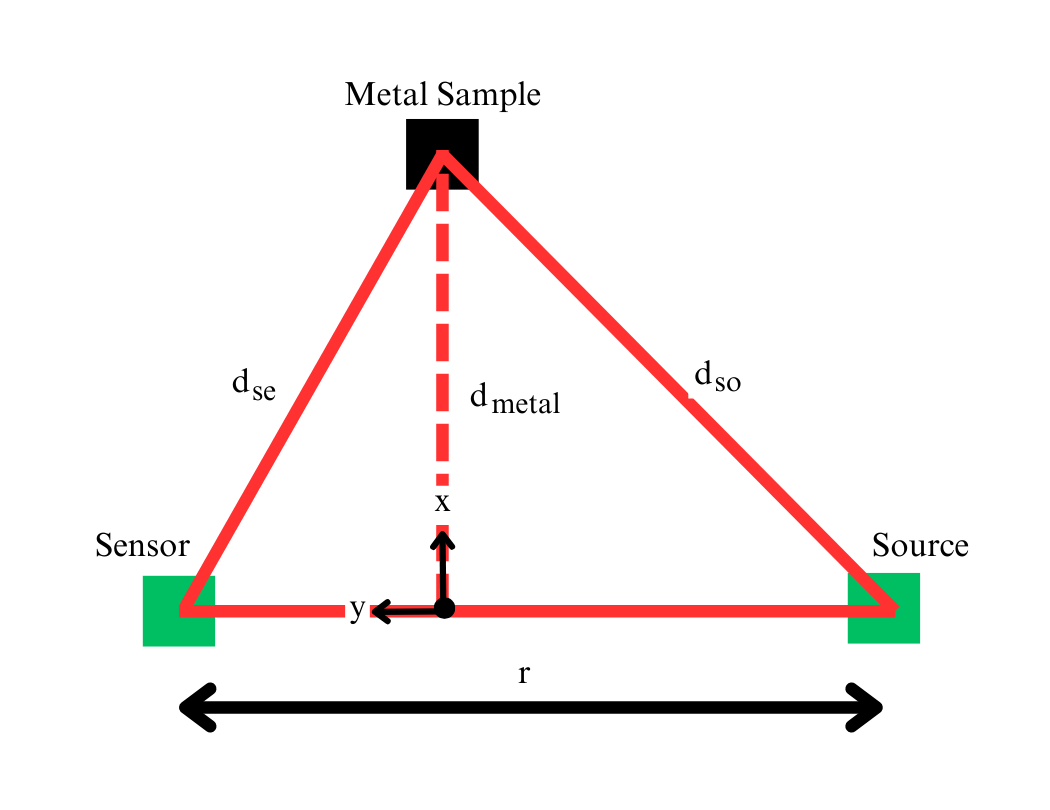
\includegraphics[width=\columnwidth]{chaic2.png}}
\caption{Simplified configuration of source, sensor and metal sample in the $xy$ plane. $d_{so}$ is the distance from the source to metal, while $d_{se}$ is from sensor to metal. In our experiments $d_\mathrm{metal}$ is the $x$ coordinate of the metal. Here the source and sensor are shown aligned on the $y$-axis, but the actual experimental setups deviate slightly, see Fig. \ref{location_example}. 
}
\label{distance_config}
\end{figure}

When metal is present, it interacts with the source field to create an interfering field proportional to the source field strength (Fig. \ref{distance_config}). The metal effectively becomes a secondary dipole source, whose strength depends on the cube of both the transmitter-to-metal distance ($d_{so}$) and the metal-to-sensor distance ($d_{se}$):
\begin{equation}
\Delta v \propto \frac{1}{d_{so}^3 d_{se}^3}
\label{eq:metal_interference}
\end{equation}

Combining these relationships, the position error due to metal interference follows:
\begin{equation}
\Delta r \propto \frac{r^4}{d_{so}^3 d_{se}^3}
\label{eq:combined_error}
\end{equation}
An important consequence of this is that the source-to-sensor distance establishes a distance scale for whether metal is "nearby" or "far away" and whether the metal is "large" enough that the dipole model becomes inaccurate.

When $r$ is held constant and $d_{metal} \gg r$ then $d_{so} \approx d_{se} \approx d_{metal}$ so in the limit of far distance:
\begin{equation}
\Delta r \propto d_{metal}^{-6}
\label{eq:dropoff_power}
\end{equation}
However, at far distance the metal effect also becomes undetectable, so the applicability of this approximation is unclear.

In summary, Equation \eqref{eq:combined_error} model makes strong simplifications to both the tracker operation (reducing three vector fields to a scalar) and also to the metal (assuming it is small enough for dipole approximation), but gives useful insight into the underlying physics.

\subsection{Mechanisms of Metal Interference}
\label{subsec:interference_mechanisms}
Metal interference in electromagnetic tracking occurs through two primary mechanisms: eddy currents and permeability effects. These mechanisms interact differently with various modulation frequencies, creating complex interference patterns that depend on material properties and geometry.

\subsubsection{Eddy Current Loop Model}
\label{subsubsec:eddy_current_model}
Eddy currents are circular electrical currents induced within conductive materials when exposed to a time-varying magnetic field. These currents generate their own magnetic fields that oppose the original field, causing distortion of the measured field at the sensor location. 
\begin{figure}[!htbp]
\centerline{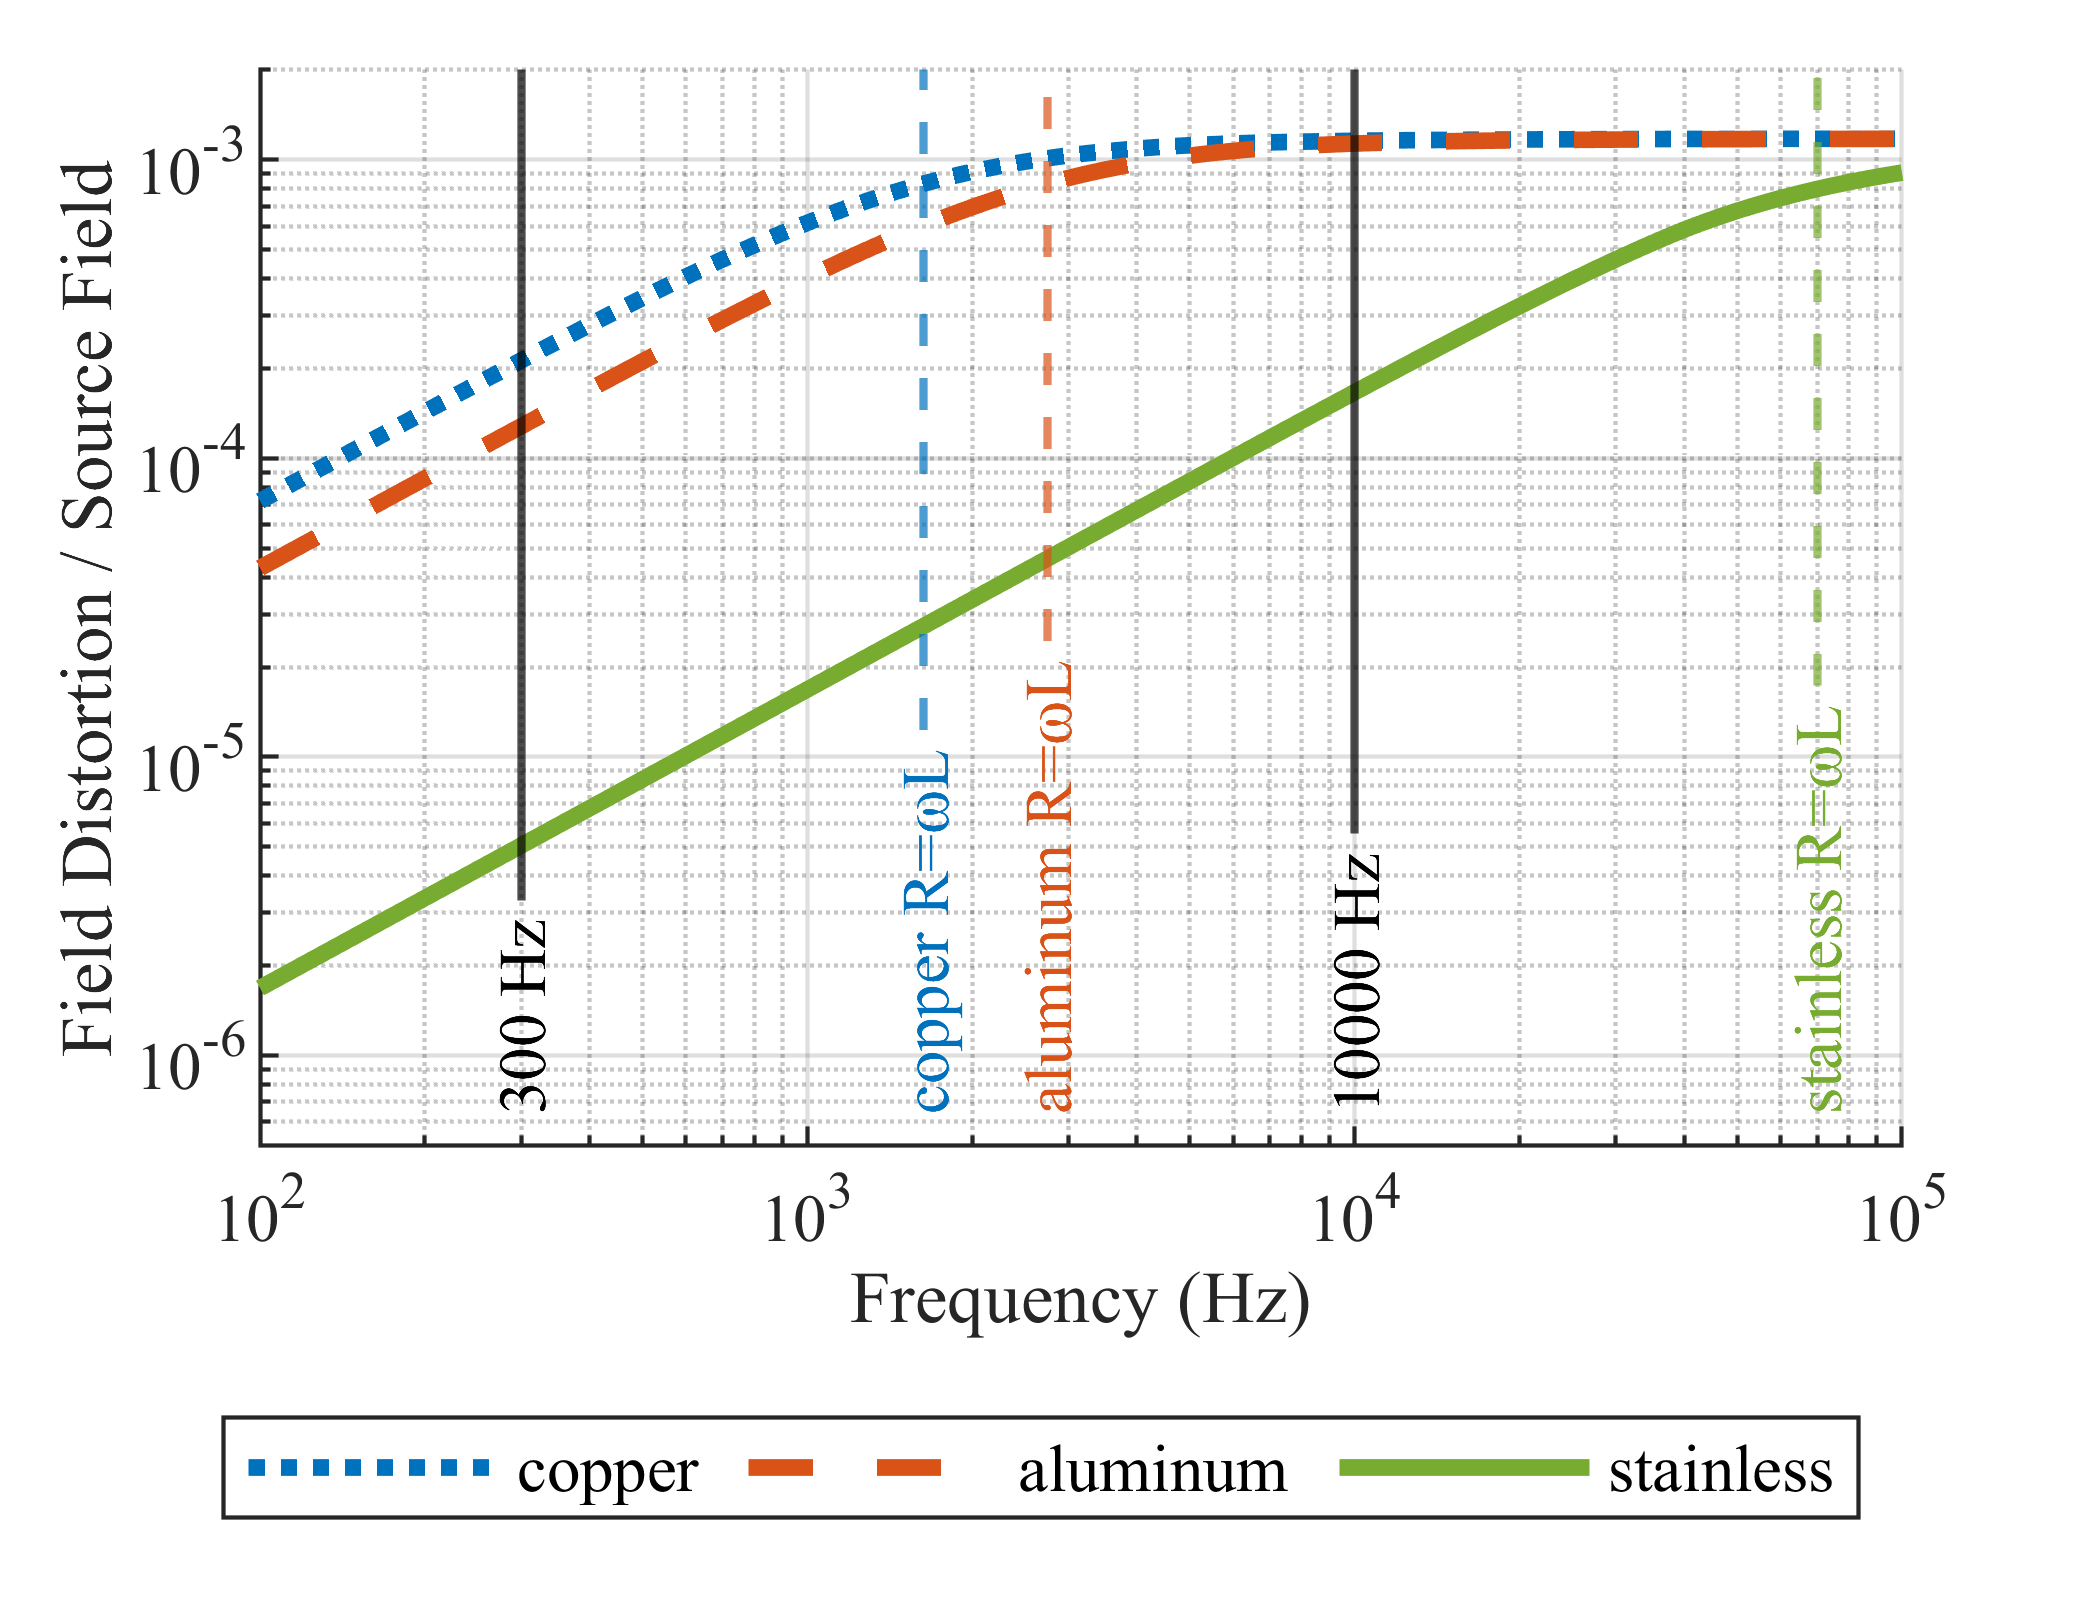
\includegraphics[width=\columnwidth]{chaic3.png}}
\caption{Eddy current frequency response modeled as a wire loop 25.0 mm diameter loop, 2.0 mm wire thickness, positioned midway between the source and sensor. Field distortion values are normalized to the source field strength at the sensor. At low frequency, the loop impedance is dominated by resistance, so the induced current increases linearly with frequency, but at higher frequencies the inductance dominates, holding the current constant. This $R = \omega L$ corner depends on the metal conductivity. For high conductivity metals eddy currents do not begin to decrease until well below the high AC modulation frequency, limiting the eddy current interference reduction.}
\label{eddy_current_freq_response}
\end{figure}

To model the frequency dependence of eddy current interference consider a simple metal loop placed midway between the source and sensor (Fig. \ref{eddy_current_freq_response}). When placed in a time-varying magnetic field, eddy currents are induced according to Faraday's law \cite{griffiths_introduction_1999}. For a sinusoidal magnetic field $B(t) = B_0 \sin(\omega t)$ with angular frequency $\omega = 2\pi f$, the induced voltage in the loop is:
\begin{equation}
V_{induced} = -\frac{d\Phi}{dt} = -\frac{d(\accentset{\rightharpoonup}{B} \cdot \accentset{\rightharpoonup}{A})}{dt} = -\omega B_0 A \cos(\omega t)
\label{eq:induced_voltage}
\end{equation}
\noindent where $A = \pi (d/2)^2$ is the loop area. The RMS value of this voltage is proportional to frequency: $V_{RMS} \propto \omega$. This voltage drives a current through the loop, which is limited by the loop's impedance. The impedance consists of the loop's resistance $R$ and inductive reactance $X_L = \omega L$:
\begin{equation}
I = \frac{V_{induced}}{\sqrt{R^2 + (\omega L)^2}}
\label{eq:loop_current}
\end{equation}
At low frequencies where $R \gg \omega L$, the current increases linearly with frequency as $I \propto \omega/R$. At higher frequencies where $\omega L \gg R$, the current approaches a constant value as $I \propto 1/L$. This transition occurs at the corner frequency $f_c = R/(2\pi L)$. For highly conductive materials like copper, this corner occurs at lower frequencies than for materials with higher resistivity such as stainless steel. The resulting distortion field is proportional to the eddy current and follows the same frequency response characteristics.

Note that the corner frequencies are tunable by the loop diameter and thickness, though we did not do so. This model also becomes inaccurate at frequencies well above our frequency range of interest where skin effect and other losses become dominant.

\subsubsection{Eddy Currents in Real Metal Objects}
In real metal objects their three-dimensional geometry defines the paths of induced eddy currents, with an effective ``loop area'' that depends  on the shape, size, and orientation of the metal object relative to the field. In rod-shaped objects, currents flow in loops perpendicular to the applied field and the rod axis, while in sheet metal, currents form larger loops with greater induced voltage. When an object is rotated, the projected area intercepting the field changes, altering the current patterns.

\subsubsection{Skin Effect}
The skin effect describes how alternating current tends to flow near the surface of a conductor. This occurs because eddy currents induced within the conductor generate magnetic fields that oppose the original field, reducing field penetration into the material. The  depth at which current density decreases to 1/e (approximately 37\%) of its surface value is called the skin depth ($\delta$) \cite{wheeler_formulas_1942}, given by:
\begin{equation}
\delta =  \sqrt{1/{\pi f \mu \sigma}}
\label{eq:skin_depth}
\end{equation}
where $\sigma$ is conductivity, $\mu$ is magnetic permeability, and $f$ is the frequency of the field. Skin depth increases with decreasing frequency, and for non-ferromagnetic materials, the skin depth at 300\,Hz is much larger than at 10\,kHz (Table \ref{material_prop}). As the skin depth approaches the metal thickness, the metal becomes increasingly transparent to the magnetic field.

\subsubsection{Permeability Effects in Ferromagnetic Materials}
Ferromagnetic materials (such as steel alloys) have a high relative permeability ($\mu_r \gg 1$), a measure of their ability to internally magnify an applied field, concentrating and redirecting the external fields measured by the sensor. Unlike eddy current effects, permeability effects often decrease with frequency \cite{bowler_frequency-dependence_2006}. This occurs because the effective permeability of ferromagnetic materials decreases at higher frequencies due to the skin effect limiting the volume of material that participates in the magnetic interaction.

The magnetic behavior of ferromagnetic objects is significantly influenced by what are known as demagnetizing fields. When placed in an external magnetic field, magnetic poles are induced on the object's surface that create their own magnetic field inside the object opposing the applied field.
The strength of demagnetizing field depends on the shape of the object and its orientation relative to the applied field \cite{prozorov_effective_2018}, characterized by the demagnetizing factor $0 \leq N_d \leq 1$ where $N_d=1$ is fully demagnetized. For a sphere, $N_d = 1/3$ in all directions, but for other objects, $N_d$ varies with orientation. A sheet oriented parallel to the field has low demagnetization ($N_d$ approaching $0$),  but if perpendicular to the field then $N_d$ approaches 1. Whether demagnetization increases or decreases interference depends on the source-sensor-metal positioning.

\subsubsection{Interaction of Multiple Interference Mechanisms}
\label{subsubsec:mechanisim_summary}
Shape and orientation dictate eddy‑current loop area; in ferromagnetic samples the same geometry also alters demagnetizing fields. For ferromagnetic metals, both eddy currents and permeability effects contribute to interference. At lower frequencies, permeability effects often dominate, while at higher frequencies, eddy current effects become more significant. These competing mechanisms contribute to the frequency response of interference from ferromagnetic metals.

\section{Methodology}
Our experiments manipulated five variables: the \textit{metal type}, \textit{shape}, \textit{position} and \textit{rotation}, and the tracker \textit{modulation}. See Table \ref{hypothesis} for an overview of the variables and our hypotheses about their influence on interference.

\subsection{Metal Types and Shapes}
\label{subsec:metal_types}
We tested six types of metal commonly present in medical applications. For EMT metal interference purposes these fall into three categories: 
\begin{itemize}
\item \textbf{Ferromagnetic metals:}\\ 
Low carbon steel (LC steel), 416 stainless steel (416 SS)

\item \textbf{Non-ferromagnetic metals with high conductivity:}\\
6061 aluminum (6061 Al), copper (Cu)

\item \textbf{Non-ferromagnetic metals with low conductivity:}\\
304 stainless steel (304 SS), titanium (Ti)
\end{itemize}

Table \ref{material_prop} summarizes the permeability, conductivity and skin depths of these materials\cite{bowler_frequency-dependence_2006,callister_notitle_2019,mitchell_notitle_2010}.
Note that while the metal types are nominally the same across the shapes, the materials will not be entirely identical. More important than any small differences in composition, different processing can have significant effects. All three shapes were likely cold worked, and then $\mu_r$ can reach $5$ or more for 304 SS.

\begin{table}[!htbp]
\caption{Relative Permeability, Conductivity, and Skin Effect at 300\,Hz and 10\,kHz  Properties for Metal Samples}
\label{material_prop}
\setlength{\tabcolsep}{3pt}
\centering
\begin{tabular}{|l|c|c|c|c|}
\hline
\parbox{45pt}{\centering {Metal Type}} & 
\parbox{25pt}{\centering {$\mu_r$}} & 
\parbox{45pt}{\centering {$\sigma$ (S/m)}} & 
\parbox{50pt}{\centering {$\delta_{300 Hz}$ (m)}} &
\parbox{50pt}{\centering {$\delta_{10\,kHz}$ (m)}}\\
\hline

LC steel& 
$240$& $6.29\times10^6$&$7.48\times10^{-4}$&$ $ \\
$ $ & $180$& $ $&$ $&$1.5\times10^{-4}$ \\

416 SS& 
$800$& $1.75\times10^6$&$7.76\times10^{-4}$&$ $ \\
$ $& $500$& $ $&$ $&$1.70\times10^{-4}$ \\

304 SS& 
$1.02$& $1.39\times10^6$&$2.44\times10^{-2}$&$4.23\times10^{-3}$ \\

6061 Al& 
$1.00$& $3.77\times10^7$&$4.73\times10^{-3}$&$8.19\times10^{-4}$ \\

Ti& 
$1.00$& $5.85\times10^5$&$3.80\times10^{-2}$&$6.58\times10^{-3}$ \\

Cu& 
$1.00$& $5.96\times10^7$&$3.76\times10^{-3}$&$6.52\times10^{-4}$ \\
\hline
\end{tabular}
\end{table}

\begin{figure}[!htbp]
\centerline{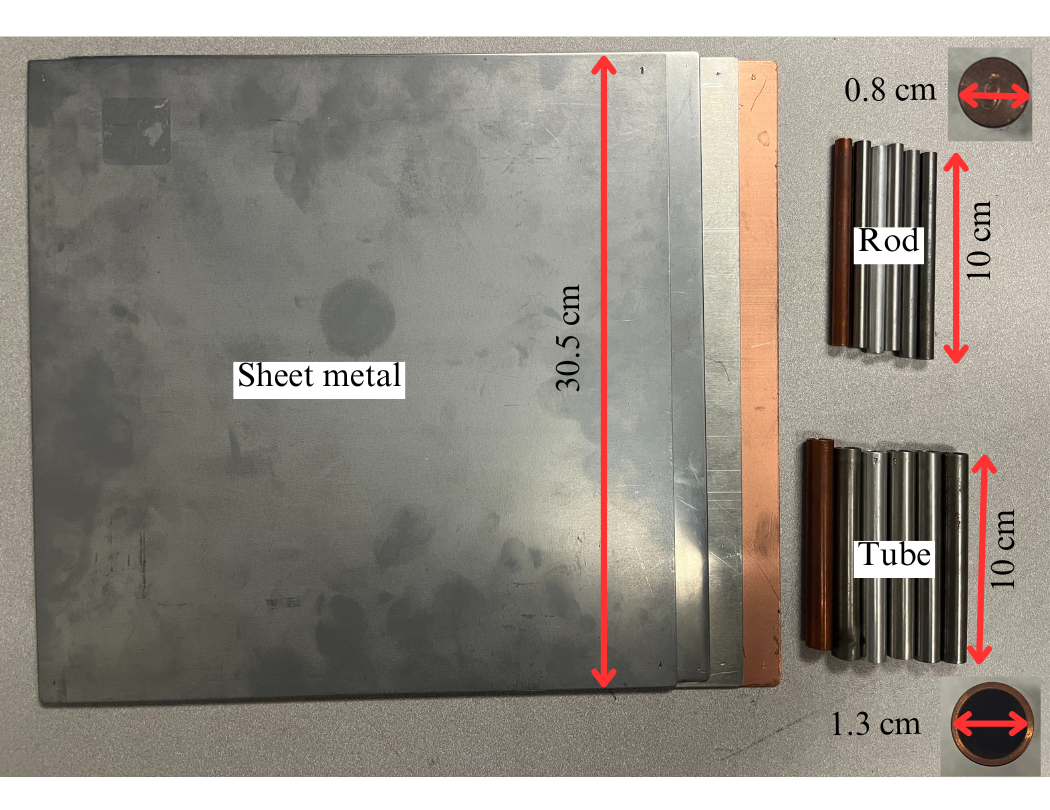
\includegraphics[width=\columnwidth]{chaic4.png}}
\caption{Metal samples are in three shapes and six metal types. The rods and tubes are both 100 mm long and both contain the same amount of metal. Insets show the end views of the rod and tube shapes.}
\label{Sample}
\end{figure}

We tested three metal shapes (Fig. \ref{Sample}):\\
\textbf{rod:}
7.9 mm diameter and 100 mm length, chosen to resemble the shape and metal content of a handheld surgical instrument.\\
\textbf{tube:}
the same length and metal volume as the rods but with an outer diameter of 12.7 mm and 1.3 mm wall thickness, allowing investigation of metal thickness.\\
\textbf{sheet:}
305 mm square with 1.3 mm thickness (matching the tube wall thickness.) Sheets were intended to represent the effect of large metal objects more distant from the workspace, such as a metal table-top. (Ti and 416 SS not tested.)


\subsection{Metal Position and Rotation}

\begin{figure}[H]
\centerline{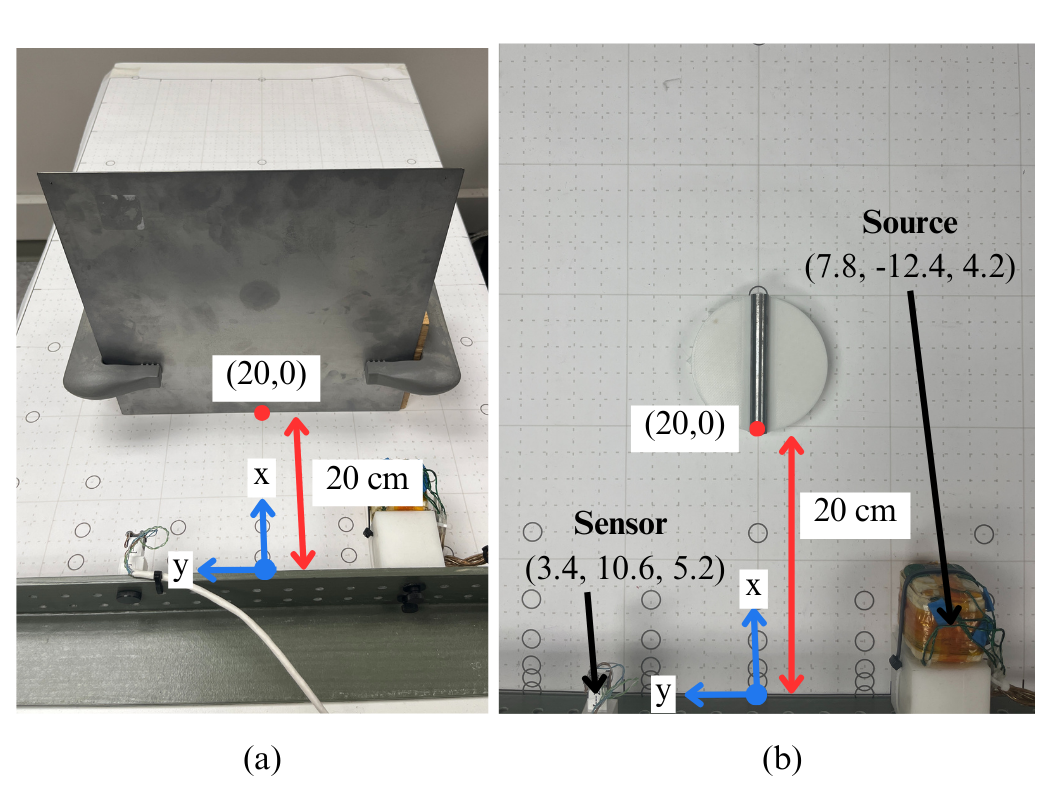
\includegraphics[width=\columnwidth]{chaic5.png}}
\caption{Experiment configuration showing the source and sensor locations and examples of metal positioned at $(20, 0)$. The metal $x$ position is measured from the nearest part, $y$ from the center. Angle is normal to the metal long axis, with (a) $0^{\circ}$ and (b) $90^{\circ}$.}
\label{location_example}
\end{figure}

Source, sensor and metal were positioned in a 100 cm $\times$ 60 cm workspace (Fig. \ref{location_example}). The source and sensor placement varied slightly between the two trackers because of the larger trakSTAR source (see supplement~\ref{supplement:tracker_configuration}), but in both cases the source-sensor distance was 23 cm, with the source at $y=+10$ cm and the sensor at $y= -12$ cm.

We moved each sample along the $x$-axis from $(0, 0)$ to $(100, 0)$ cm, and in $y$ from $(20, -25)$ to $(20, 25)$. The effect of metal was measured by comparison to metal-free measurements recorded at the beginning and end of each move sequence.

\subsection{Modulation}
We tested three modulations (Low AC, High AC, and Pulse) using the two trackers (ILEMT and trakSTAR), see \S\ref{subsec:tested_emts}. ILEMT captures both AC modulations simultaneously, while trakSTAR required a separate data collection of all variables.

\section{Results and Discussion}

\begin{table*}[!htbp]
\caption{Experimental Variables, Summary of Hypotheses and Results}
\label{hypothesis}
\setlength{\tabcolsep}{3pt}
\centering
\begin{tabular}{|p{90pt}|p{200pt}|p{200pt}|}
\hline
Variable& 
Hypothesis& 
Results\\
\hline
Metal position& 
$\bullet$ Translation and rotation errors will be proportional to the metal-induced field change &
$\bullet$ 6-DOF pose solution introduces complex effects such as notches. Coupling error shows the simpler field change. \\

$ $&
$\bullet$ Interference will decrease as $\Delta{r} \propto d_{metal}^{-6}$ & 
$\bullet$ Exponent varies from -3 to -6\\

$ $&
$\bullet$ Interference level will vary by metal and shape, but the decrease curve will be the same. &
$\bullet$ Ferromagnetic and non-ferromagnetic curves differ, sheet vs. rod/tube differ \\

$ $&
$\bullet$ Y motion will show two peaks near source and sensor &
$\bullet$ Unexpected interaction with metal type and modulation, curves vary\\
\hline

Metal type& 
$\bullet$ Low conductive non-ferromagnetic will have least interference, nearly disappearing with low frequency modulation& 
$\bullet$ Confirmed, but near disappearance seen only when skin depth much greater than thickness.\\
$ $&
$\bullet$ Ferromagnetic and non-ferromagnetic metals will interact similarly with the spatial variables (position, shape, rotation). &
$\bullet$ Metal type affects the position curves and interacts strongly with rotation for sheets.\\
\hline

Modulation& 
$\bullet$ Pulse and low AC will show less interference relative to high AC for non-ferromagnetic metals (reverse for ferromagnetic)& 
$\bullet$ Confirmed, but difference lower than $10\,\mathrm{kHz}/300\,\mathrm{Hz}$ for high conductivity metals and higher for low conductivity\\
$ $&
$\bullet$ Pulse and low AC will be similar &
$\bullet$ Confirmed\\
\hline

Metal shape& 
$\bullet$ Sheet samples (large) will show high interference& 
$\bullet$ Confirmed, but unexpected interactions with modulation, metal type and rotation\\

$ $& 
$\bullet$ Thin ($\ll$ skin depth) tube and sheet non-ferromagnetic samples will show little interference at low frequency& 
$\bullet$ Thinness has some effect, but tubes often had larger interference than rods, regardless of modulation\\

\hline
Metal rotation& 
$\bullet$ Modest changes in the level of interference, no interaction with modulation, type or shape& 
$\bullet$ Large interaction with metal type and modulation for sheet shapes\\

\hline
\end{tabular}
\end{table*}

\begin{figure*}[!b]
\centerline{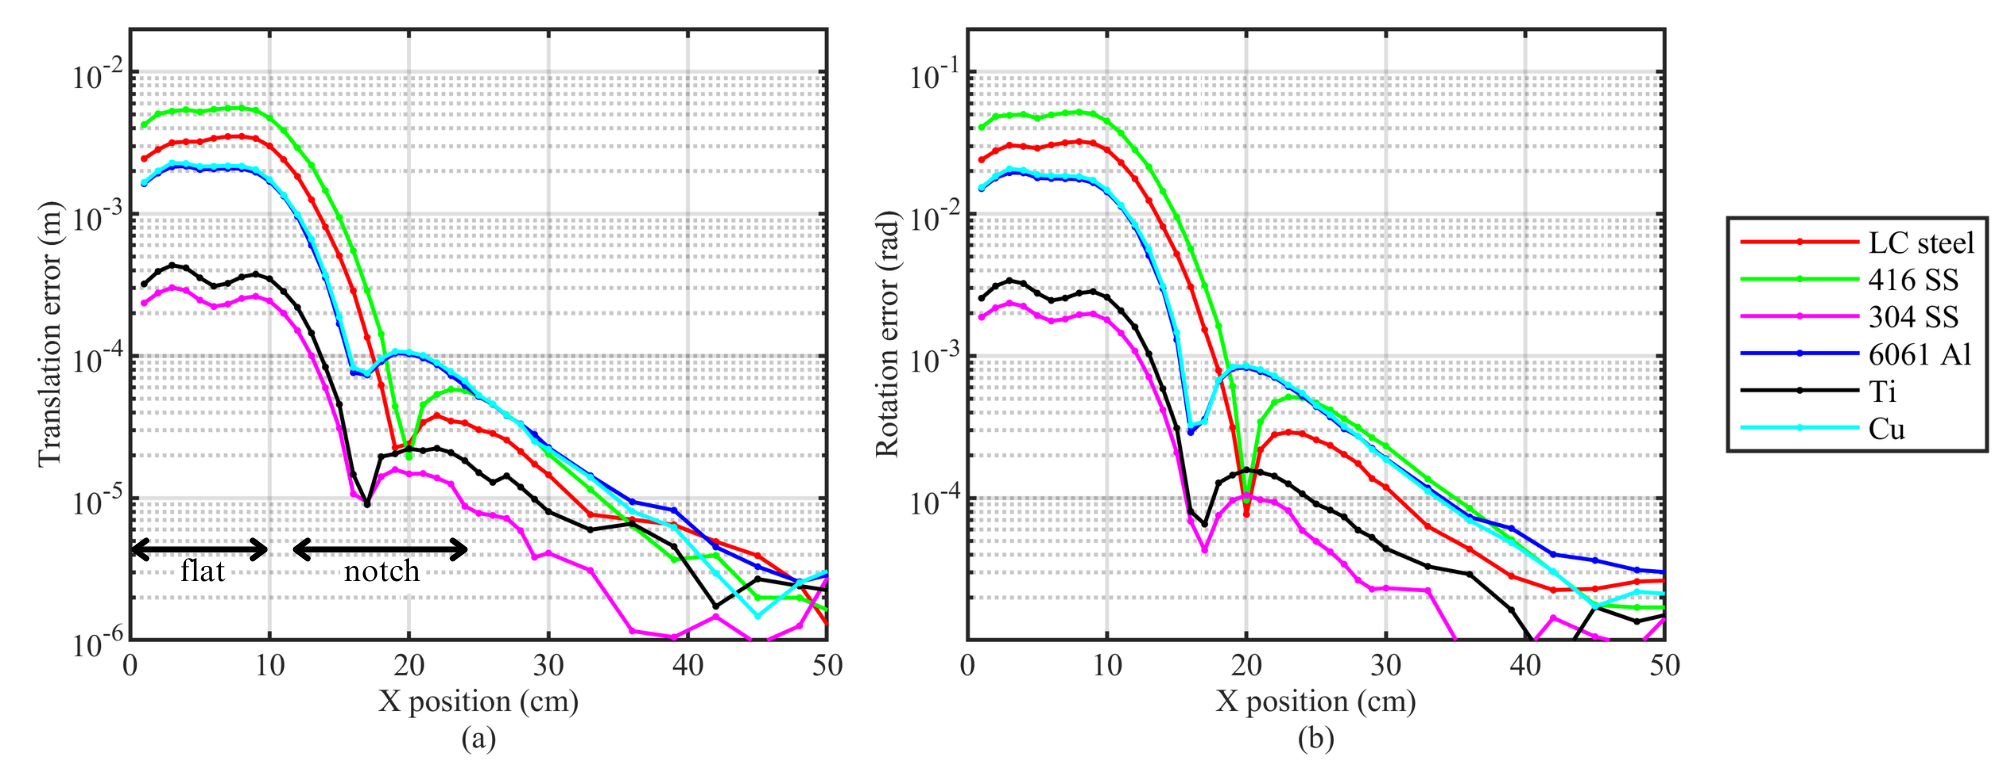
\includegraphics[width=\textwidth]{chaic6.png}}
\caption{Change in error caused by a metal tube as it is moved along the $x$ axis (normal to and away from from the source-sensor axis, Fig. \ref{location_example}). The curve shape of translation error (a) and rotation error (b) are nearly identical, as are the curve shapes across the metals. But this shape does not obey the Eqn. \eqref{eq:combined_error} prediction of monotonic decrease in error. The ILEMT detection limit is below $5 \times 10^{-6}$ m. (Modulation: High AC, Rotation: $0^\circ$)}
\label{hollow_high_xmoving}
\end{figure*}

Table \ref{hypothesis} reviews the experimental variables and our hypotheses from literature review and theory, and also briefly previews the results. Since we test five variables and many of those show interactions under certain test conditions, we will describe the effects in the order of Table \ref{hypothesis}, which progresses from the largest and most easily interpreted effects to the more subtle and context-dependent. 

\subsection{Effect of Metal Position}

\subsubsection{X motion}
Fig. \ref{hollow_high_xmoving} shows the translation and rotation error as a tube sample is moved away along the $x$-axis. Error is greatest near the source-sensor axis ($x \approx 5$ cm), then drops into a notch before increasing again. Only when $x > 25$ cm do we observe the expected power law drop-off. Error stops declining when it reaches the measurement limit near $5 \times 10^{-6}$ m.

The rotation and translation error curves are extremely similar, which is unsurprising given that the magnetics underlying EMTs implicitly create a measurement in polar coordinates. The scale factor implies a measurement at $r\approx 10$ cm, approximately $1/2$ the source-sensor distance, suggesting that the pose solution divides the error equally between rotation and translation. This simple relation was seen in all tests, so we will not present any more rotation error data.

\begin{figure}[!htpb]
\centerline{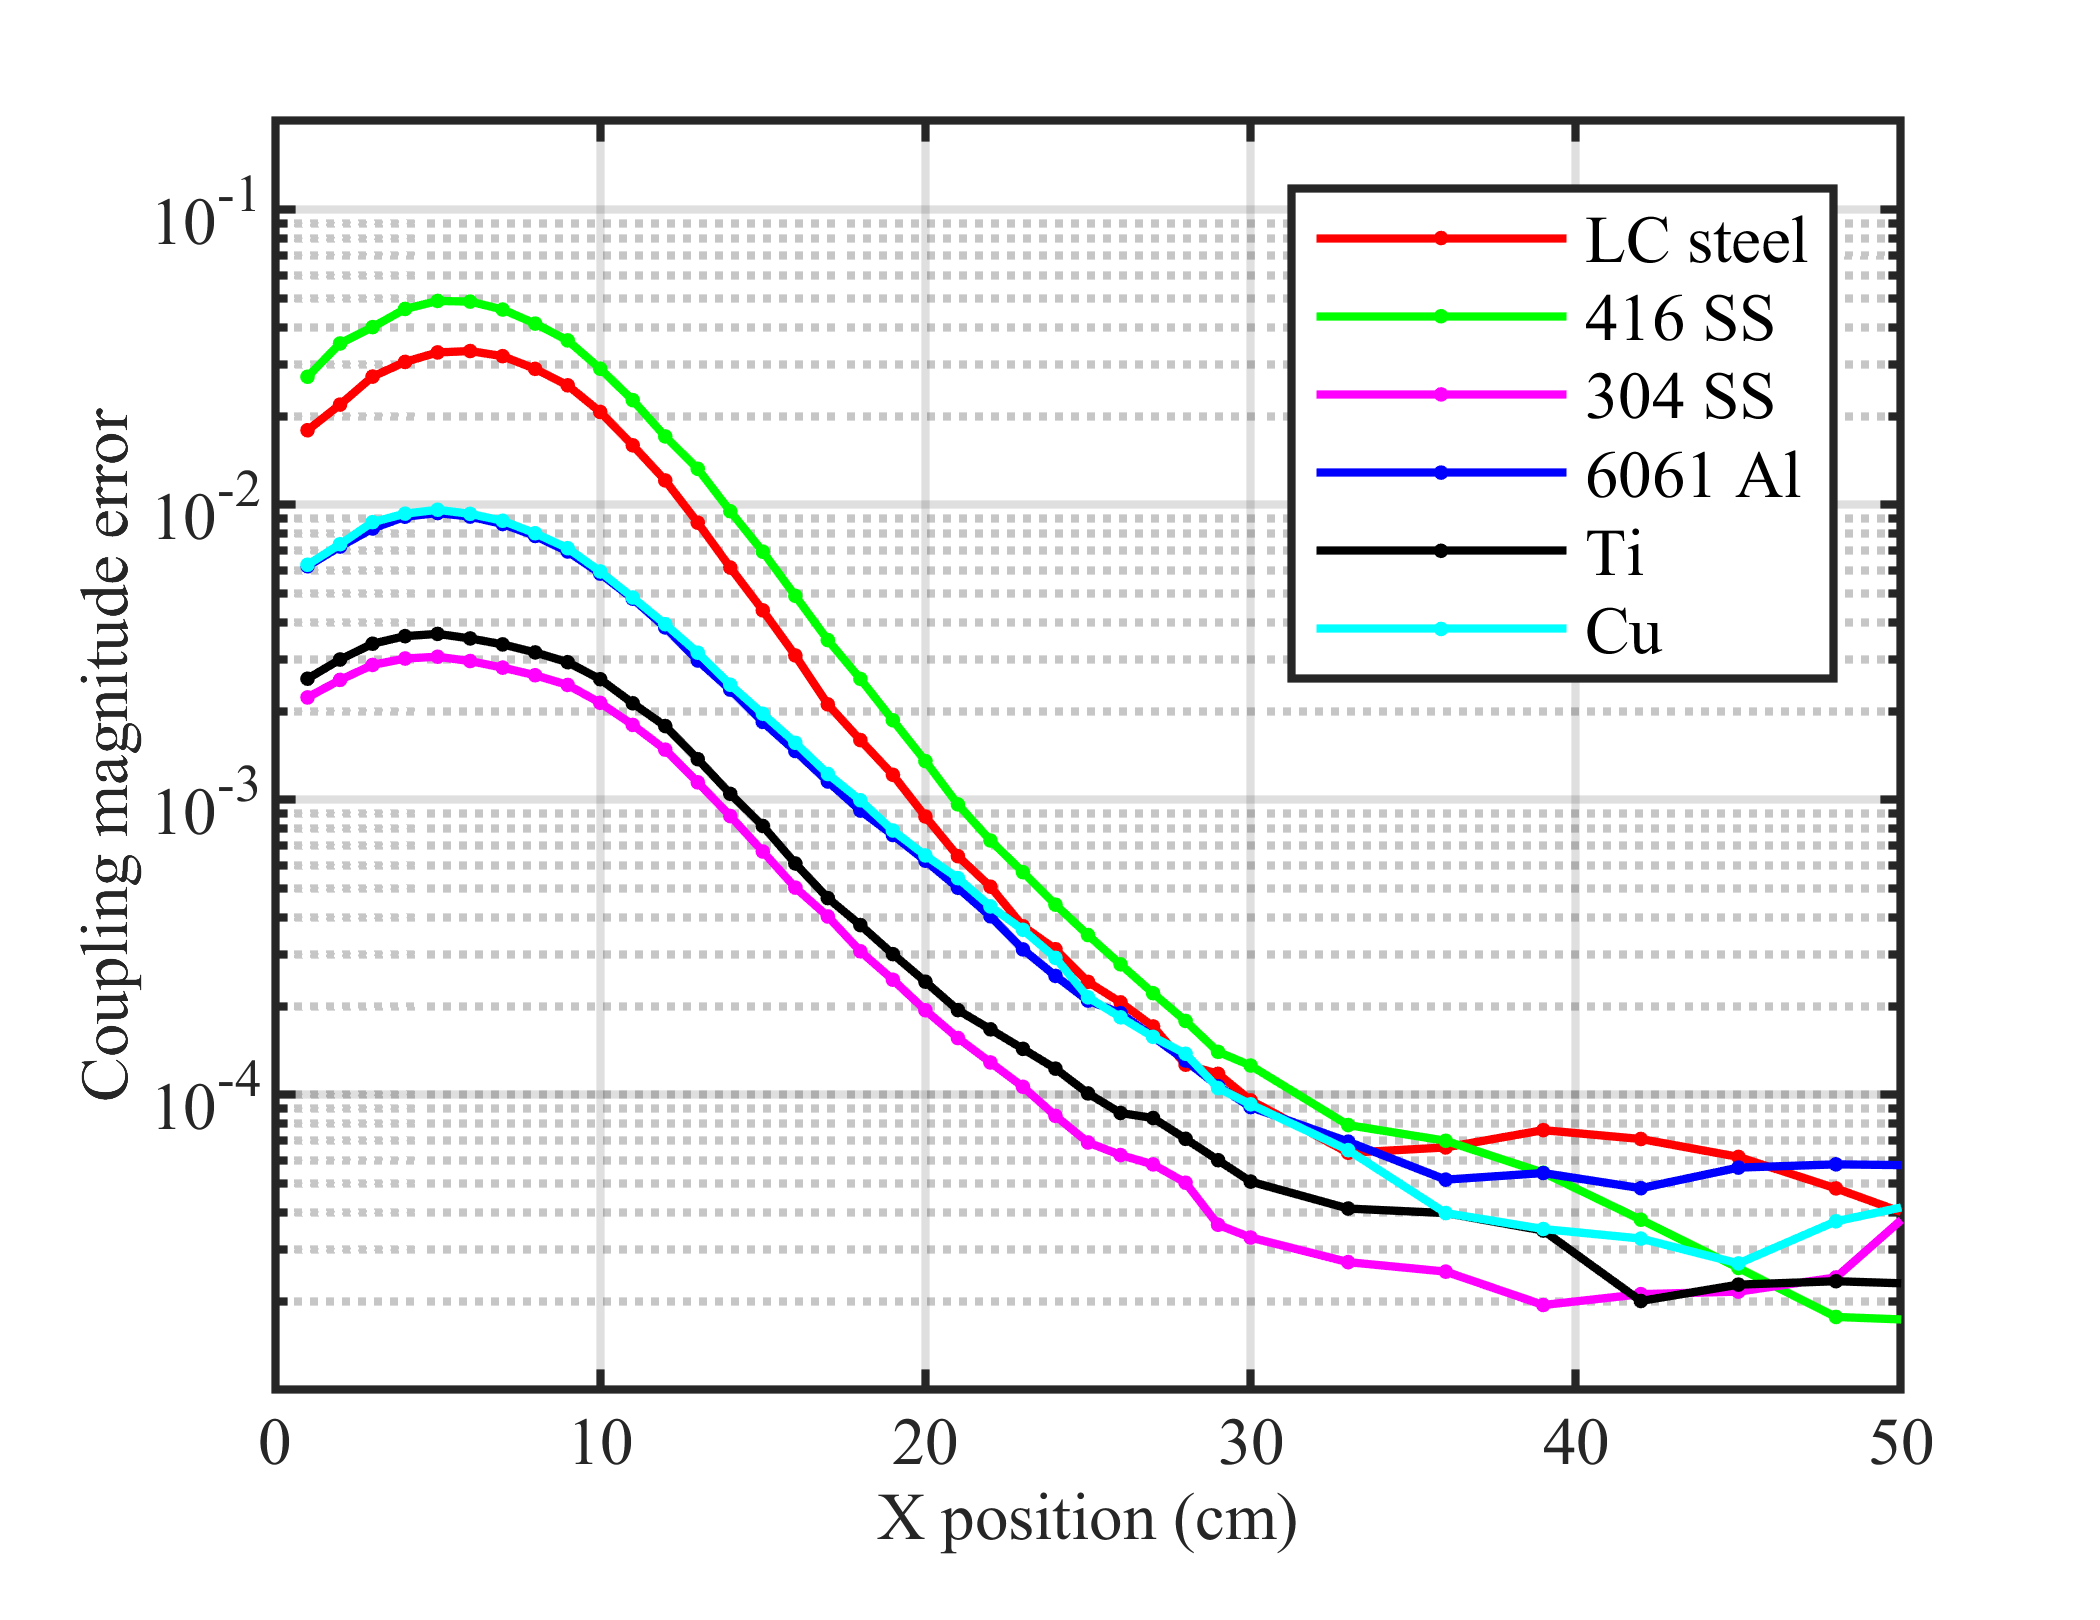
\includegraphics[width=\columnwidth]{chaic7.png}}
\caption{Coupling magnitude error is the magnitude of the magnetic change in the sensor field, before pose solution, see \S\ref{subsec:coupling}. This lacks the flat and notch features noted in Fig. \ref{hollow_high_xmoving} under the same conditions, so these deviations are caused by the pose solution algorithm's response to the change in the source vector fields (not modeled by \eqref{eq:combined_error}.)}
\label{xmoving_coupling}
\end{figure}

Although notches appear in the Fig. \ref{hollow_high_xmoving} translation and rotation error plots, in Fig. \ref{xmoving_coupling}, the coupling magnitude error (\S\ref{subsec:coupling}) forms a continuous curve, more closely corresponding to the physically expected field change from models such as \eqref{eq:combined_error}. Given the complexity of the pose solution, which maps the 9-DOF coupling to the 6-DOF pose by inverting a nonlinear magnetic model, the Nixon model's assumption (\S\ref{nixon_model}) that pose error is proportional to magnetic field change is a very rough approximation. As will be discussed in \S\ref{sec:Power Law}, in the far distance both pose error and coupling magnitude error show the same power law drop-off, but by then the error is in any case quite small, and likely below the detection limit for most EMTs, having lower resolution that ILEMT.


\begin{figure}[!tb]
\centerline{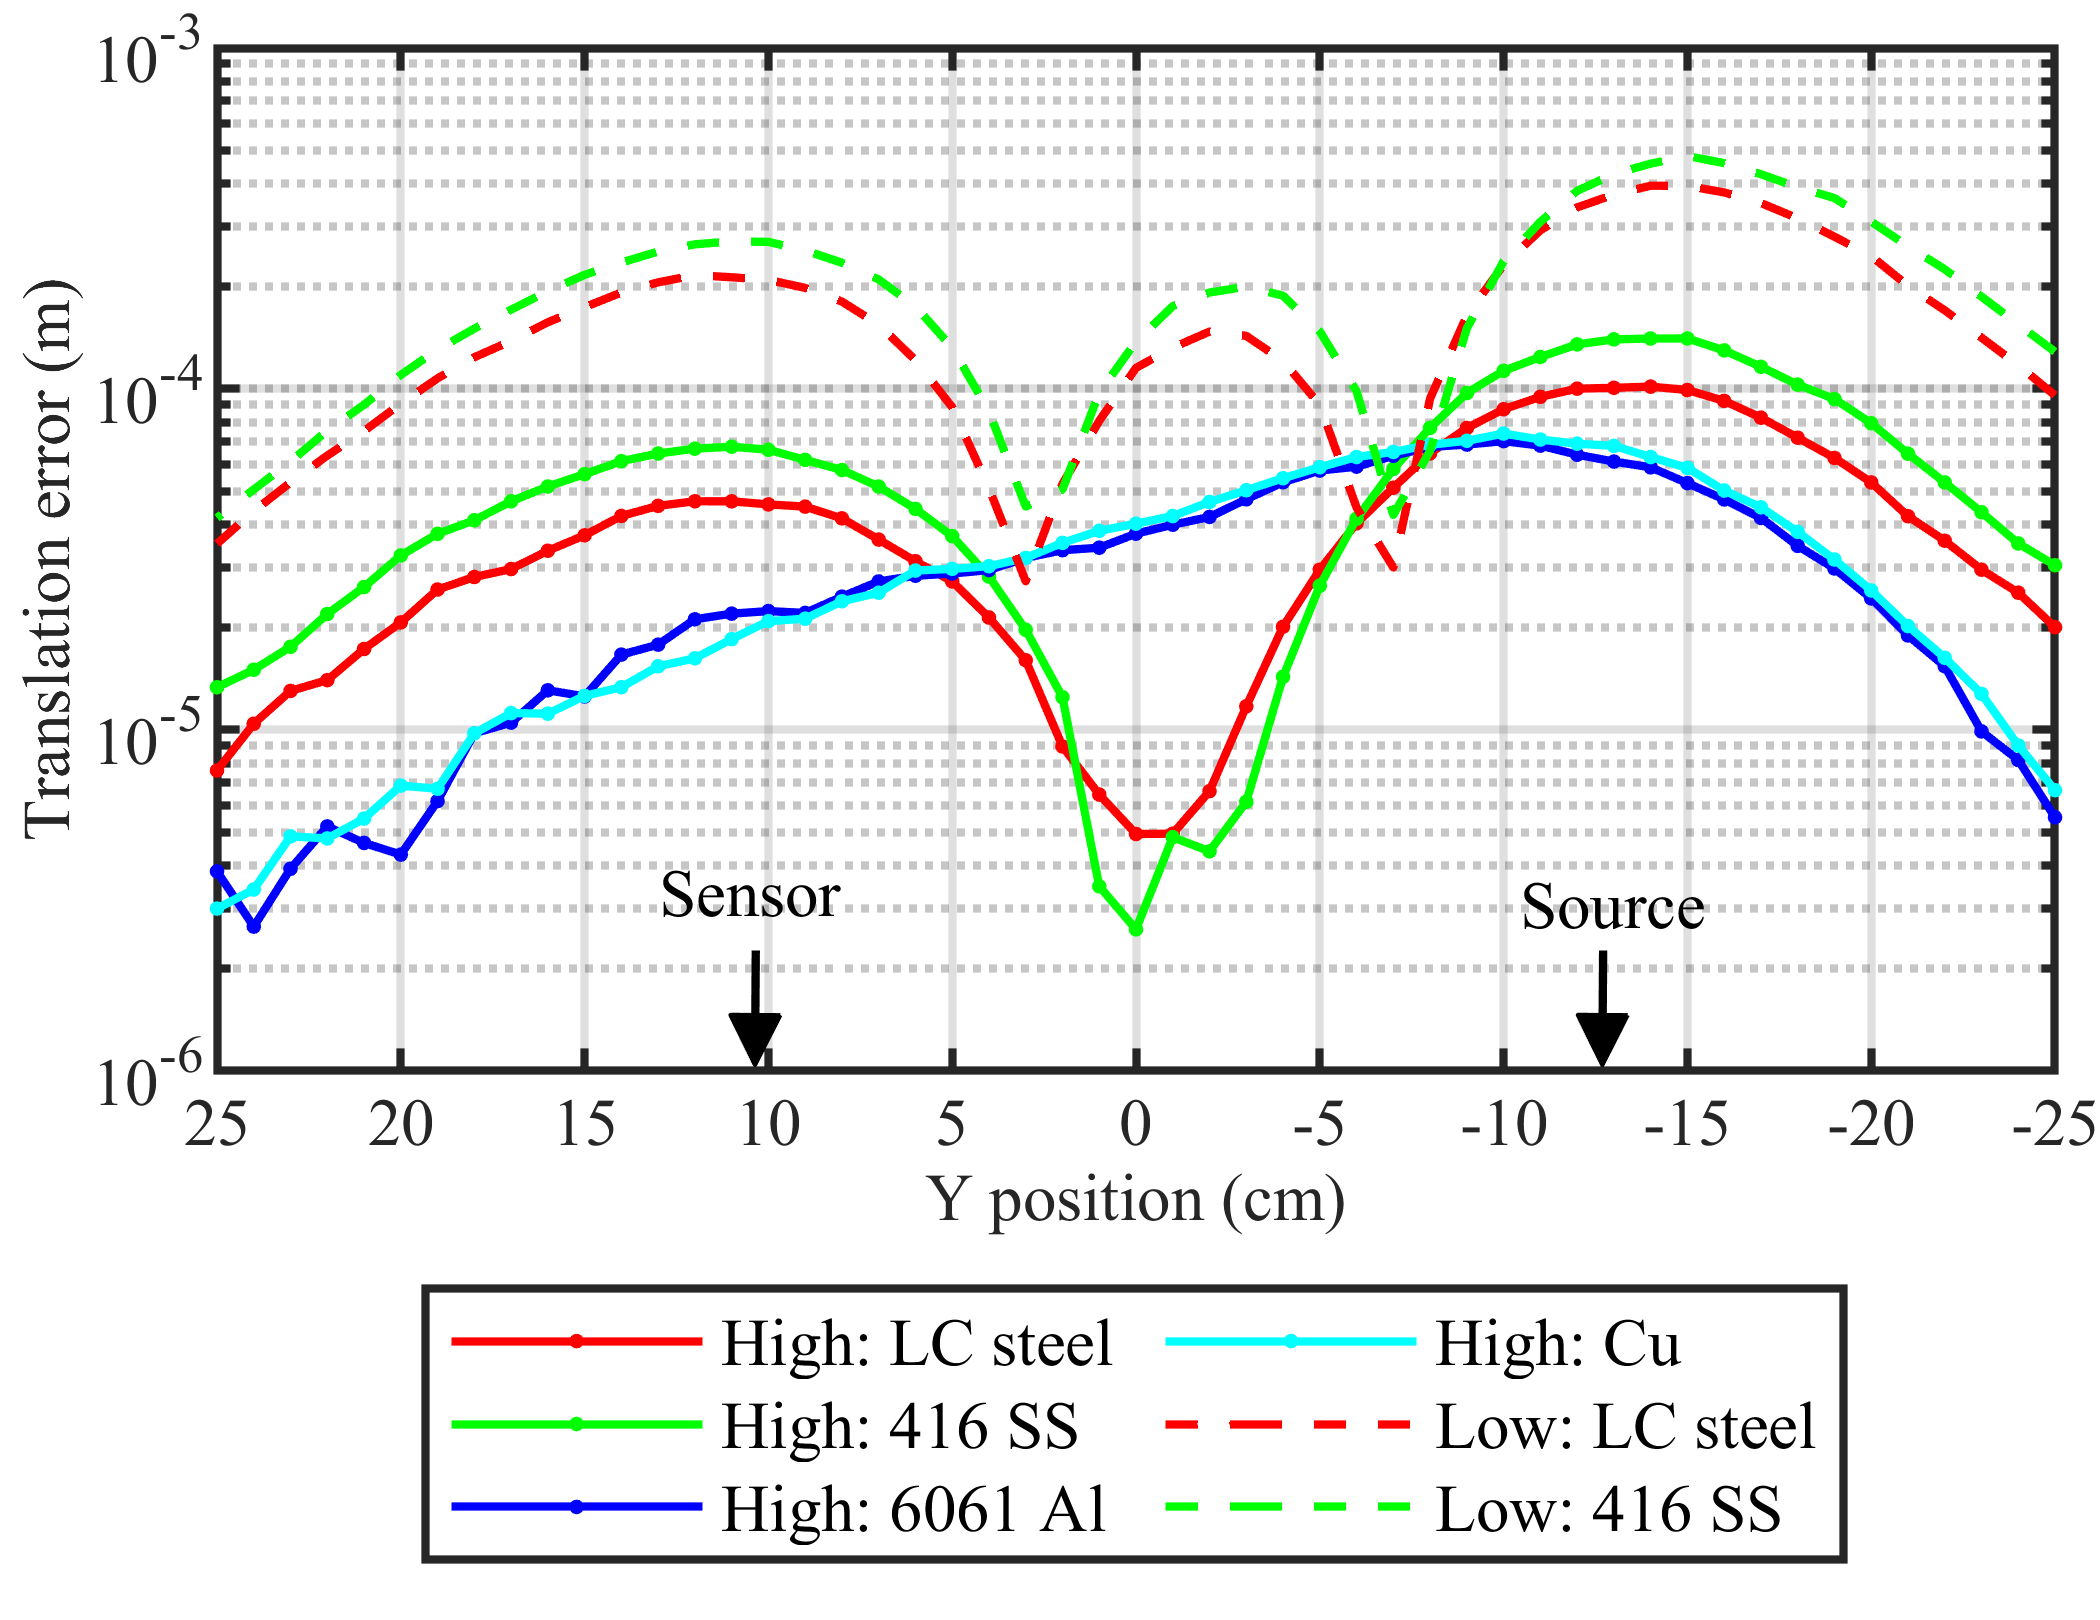
\includegraphics[width=\columnwidth]{chaic8.png}}
\caption{Translation error as a rod sample is moved in $y$ at $x = 20$ cm. We see expected peaks when metal is nearest the source and sensor, but in a dramatic interaction with metal type and modulation, there are three quite different curves. The non-ferromagnetic samples are undetectable by Low AC modulation at $x=20$ cm, and are not shown.
(Modulations: High and Low AC, Rotation: $0^\circ$)}
\label{ymoving_transrot}
\end{figure}

\subsubsection{Y motion}
 Fig. \ref{ymoving_transrot} shows translation error as a rod sample is moved parallel to the $y$ axis at $x = 20$ cm. This motion parallels the source-sensor axis (see Fig. \ref{location_example}). We do see that error peaks when the metal is nearest to the source and sensor, which is widely reported \cite { nixon_effects_1998, milne_accuracy_1996}, and predicted by the Nixon model (\S\ref{nixon_model}), but the curves vary greatly due to interactions with metal type and modulation.
 
\subsection{Effect of Metal Type}
Returning to Figs. \ref{hollow_high_xmoving}, \ref{xmoving_coupling}, in this condition (Shape: Tube, Modulation: High AC, Rotation: $0^\circ$), we can clearly distinguish the three groups of metals. In order of decreasing interference are ferromagnetic metals, then non-ferromagnetic metals having high and low conductivity (see \S\ref{subsec:metal_types}). Non-ferromagnetic metals interfere only via eddy currents, and lower conductivity \textit{usually} reduces eddy currents (see \S\ref{subsubsec:eddy_current_model}), so we expect to see the low conductivity non-ferromagnetic metals at the bottom. Higher interference from 416 SS vs. LC steel can be explained by the significant difference in permeability (see Table \ref{material_prop}.) It is common to see ferromagnetic metals as causing the greatest interference, but we do not observe this in some other conditions below, due to interactions with shape and rotation. 

Returning to Fig. \ref{ymoving_transrot}, the non-ferromagnetic metals show a significantly different response curve, without any decrease when the metal is midway between the source and sensor. But permeability effects and eddy currents modify the field directions in different ways (see \S\ref{subsubsec:mechanisim_summary}). With the complex field dependence of the pose solution algorithm, it is not entirely surprising to see qualitatively different behavior with ferromagnetic metals.

\subsection{Effect of Modulation}

Due to the frequency dependence of the eddy current and permeability metal interference mechanisms (\S\ref{subsec:interference_mechanisms}), we expect the different frequency content of the tracker modulations to create different interference effects. Summarizing the tracker modulations from \S\ref{subsec:tested_emts}, the High AC modulation is near 10\,kHz, while the Low AC and Pulse modulations are near 300\,Hz. In comparison to High AC modulation, we expected Low AC and Pulse modulations would have similar interference susceptibilities, with non-ferromagnetic metal interference decreasing greatly due to lower induced voltages generating smaller eddy currents, while ferromagnetic interference would increase somewhat due to greater permeability at low frequencies (see Table \ref{material_prop}).

\subsubsection{AC Modulation}
Fig. \ref{frequency_tube} shows the drop-off of interference during $x$ motion for both the High AC and Low AC modulation. The changes in interference between modulations are largely as expected. At a reduced frequency, the ferromagnetic metal interference increases due to increased permeability, while interference for the other metals decreases due to reduced eddy currents. But note how at High AC the high conductivity metals Cu and 6061 Al show identical interference despite their different conductivity (Table \ref{material_prop}) because the eddy currents are inductance limited (Fig. \ref{eddy_current_freq_response}), while the lower conductivity 6061 Al shows a distinctly lower interference at Low AC. For the high conductivity Cu the interference reduction is also relatively modest (see Table \ref{tab:distortion_ratios}.)

\begin{figure}[H]
\centerline{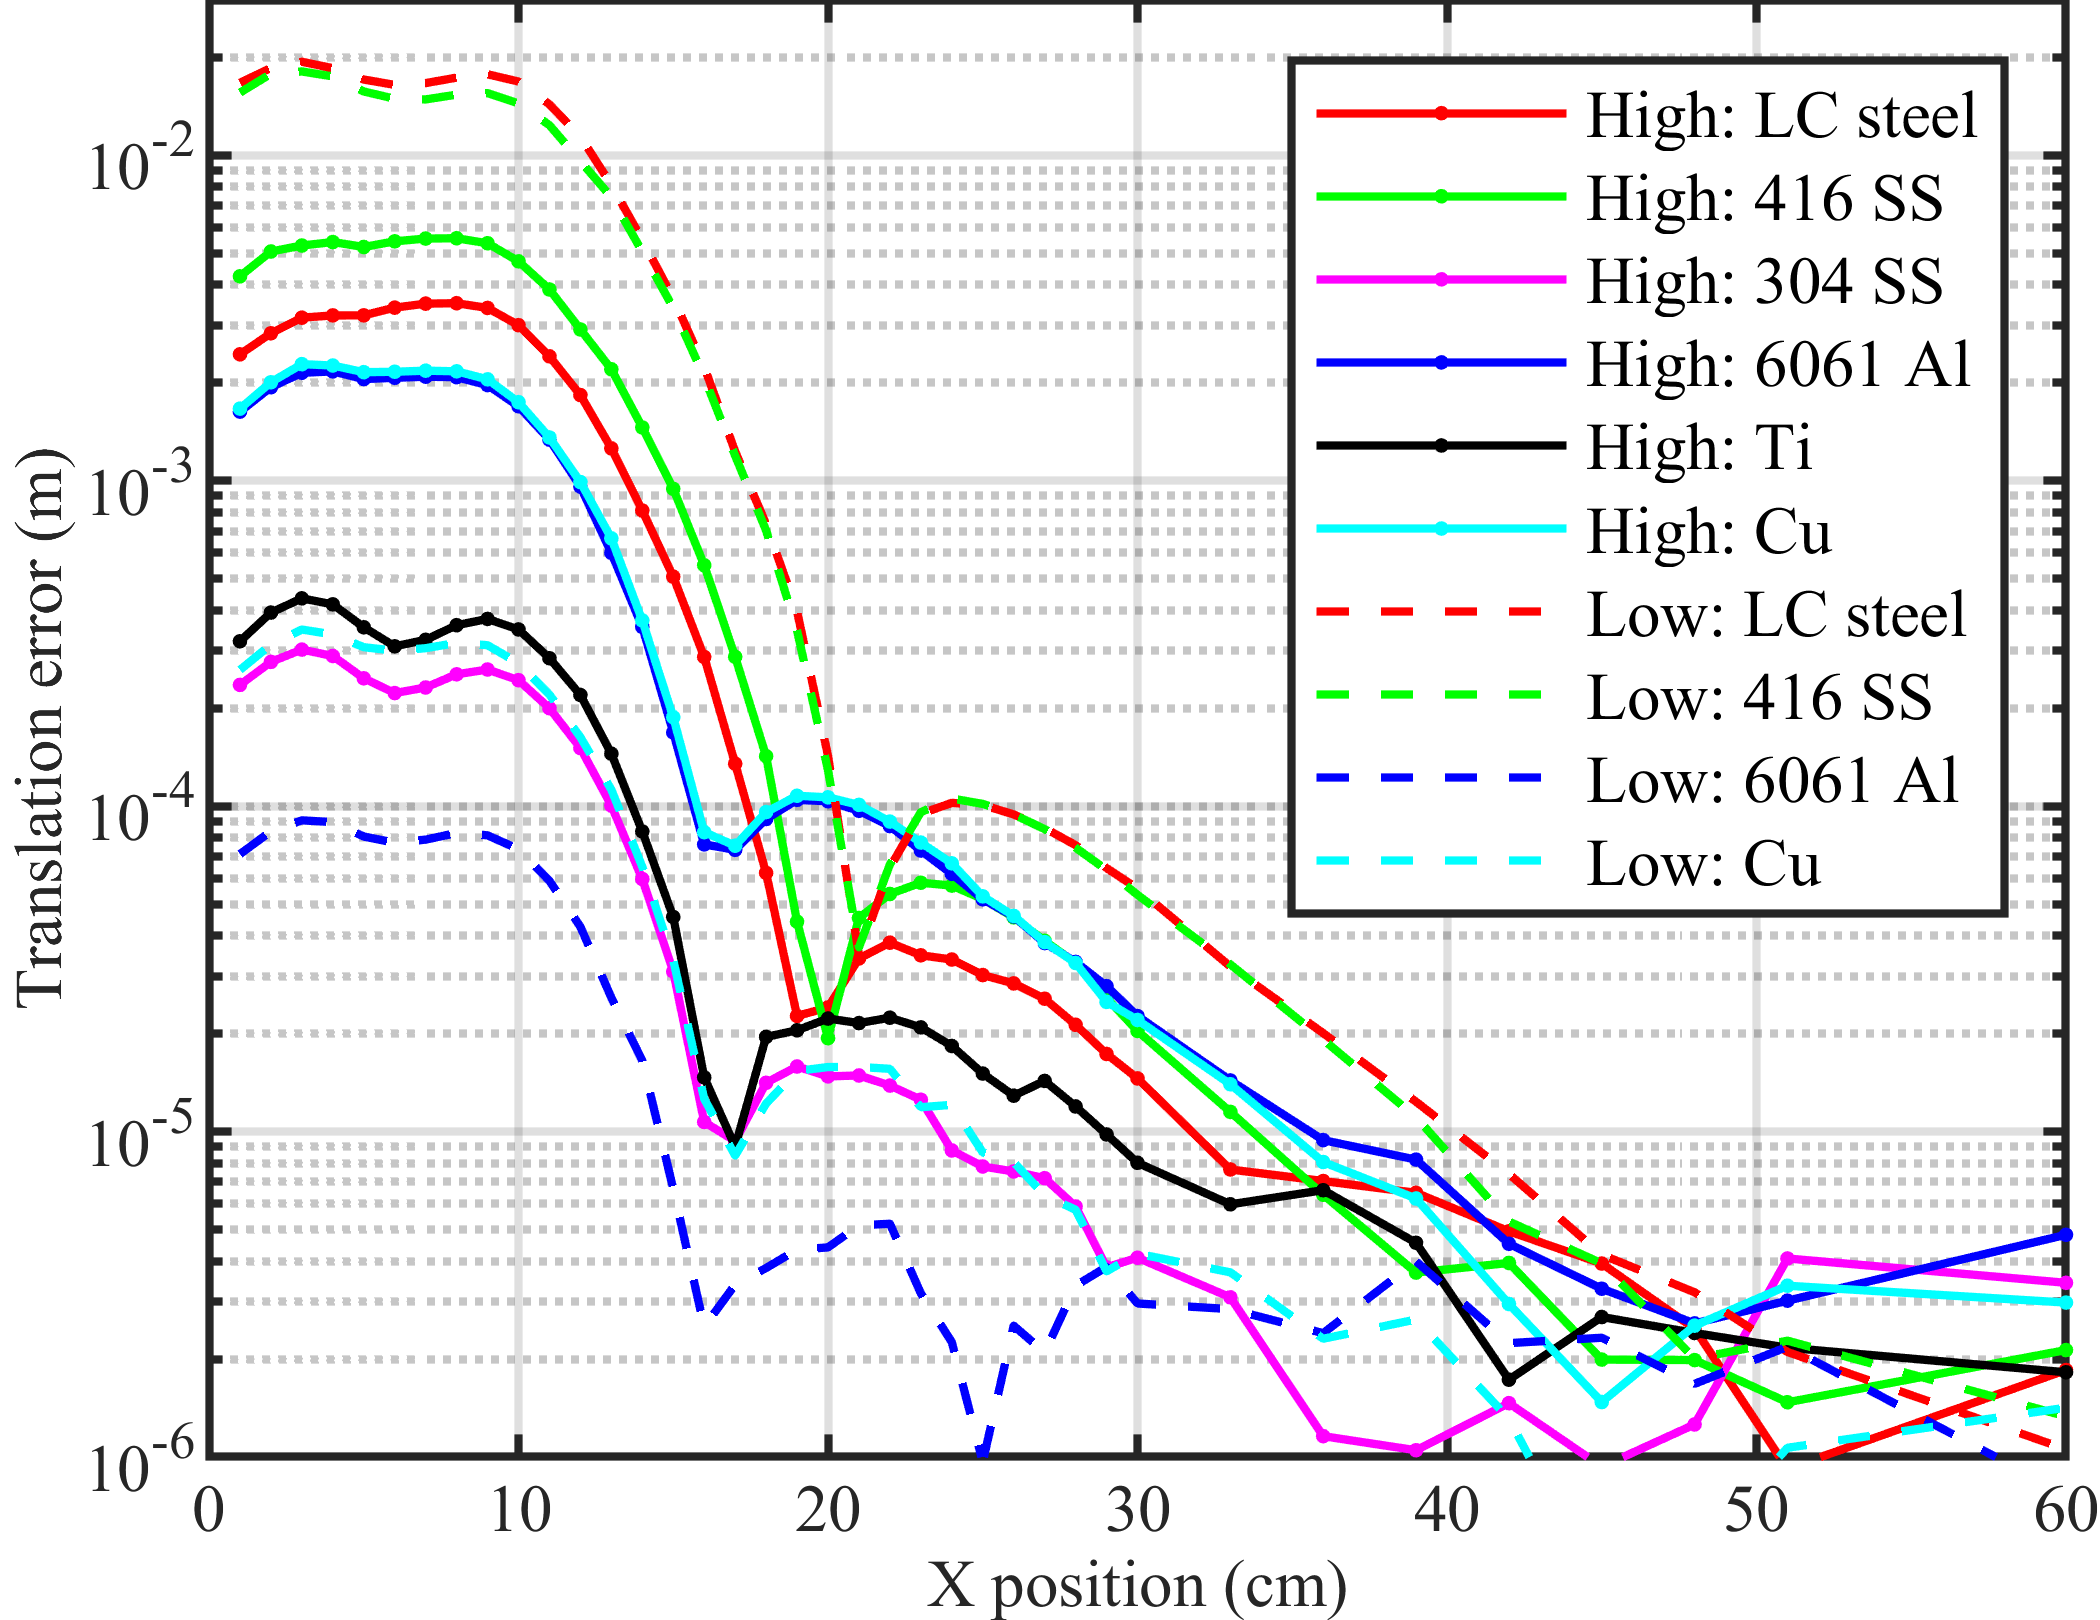
\includegraphics[width=\columnwidth]{chaic9.png}}
\caption{Translation error of tube samples during $x$ motion, comparing High AC and Low AC modulations. At a reduced frequency, the ferromagnetic metal interference increases due to increased permeability, while interference for the other metals decreases due to reduced eddy currents. The low-conductivity Ti and 304 SS are nearly undetectable using Low AC modulation, and are not shown. 
(Modulations: High and Low AC, Shape: Tube, Rotation: $0^\circ$)}
\label{frequency_tube}
\end{figure}

\begin{figure}[!tb]
\centerline{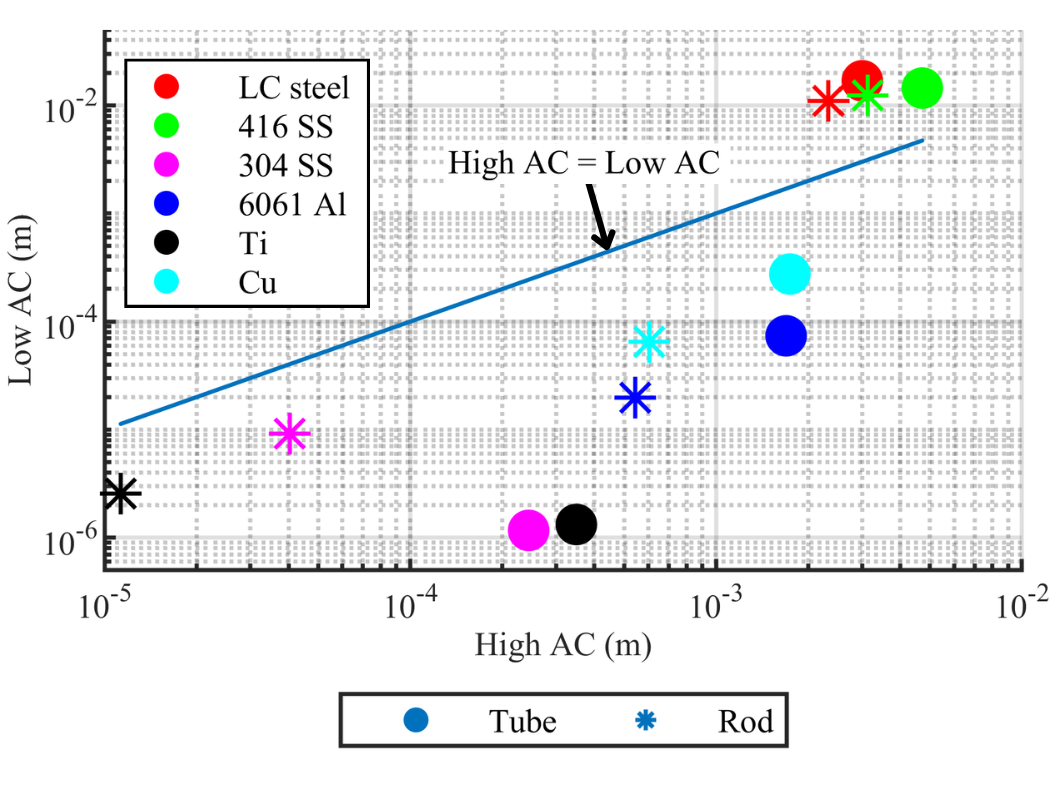
\includegraphics[width=\columnwidth]{chaic10.png}}
\caption{Scatter plot of translation error, comparing High AC and Low AC modulations. Samples above the line have greater interference at Low AC (ferromagnetic metals) while samples below the line (non-ferromagnetic) have reduced interference. The low conductivity Ti and 304 SS are near the detection limit at Low AC. The effect of rod vs. tube shape is material dependent.
(Modulations: High and Low AC, Shapes: Tube and Rod, Position: (10, 0), Rotation: $0^\circ$)}
\label{HighLow_compare}
\end{figure}

Fig. \ref{HighLow_compare} more clearly visualizes the modulation effect on error seen in Fig. \ref{frequency_tube} by plotting the high and low frequency errors for each sample at $x=10$ cm (where interference is greatest). The split effect of modulation frequency on ferromagnetic vs. non-ferromagnetic metals is clear, with ferromagnetic metals showing a significant increase in interference at low frequency, while the other metals decrease. 



\subsubsection{Pulse Modulation}

\begin{figure}[!htbp]
\centerline{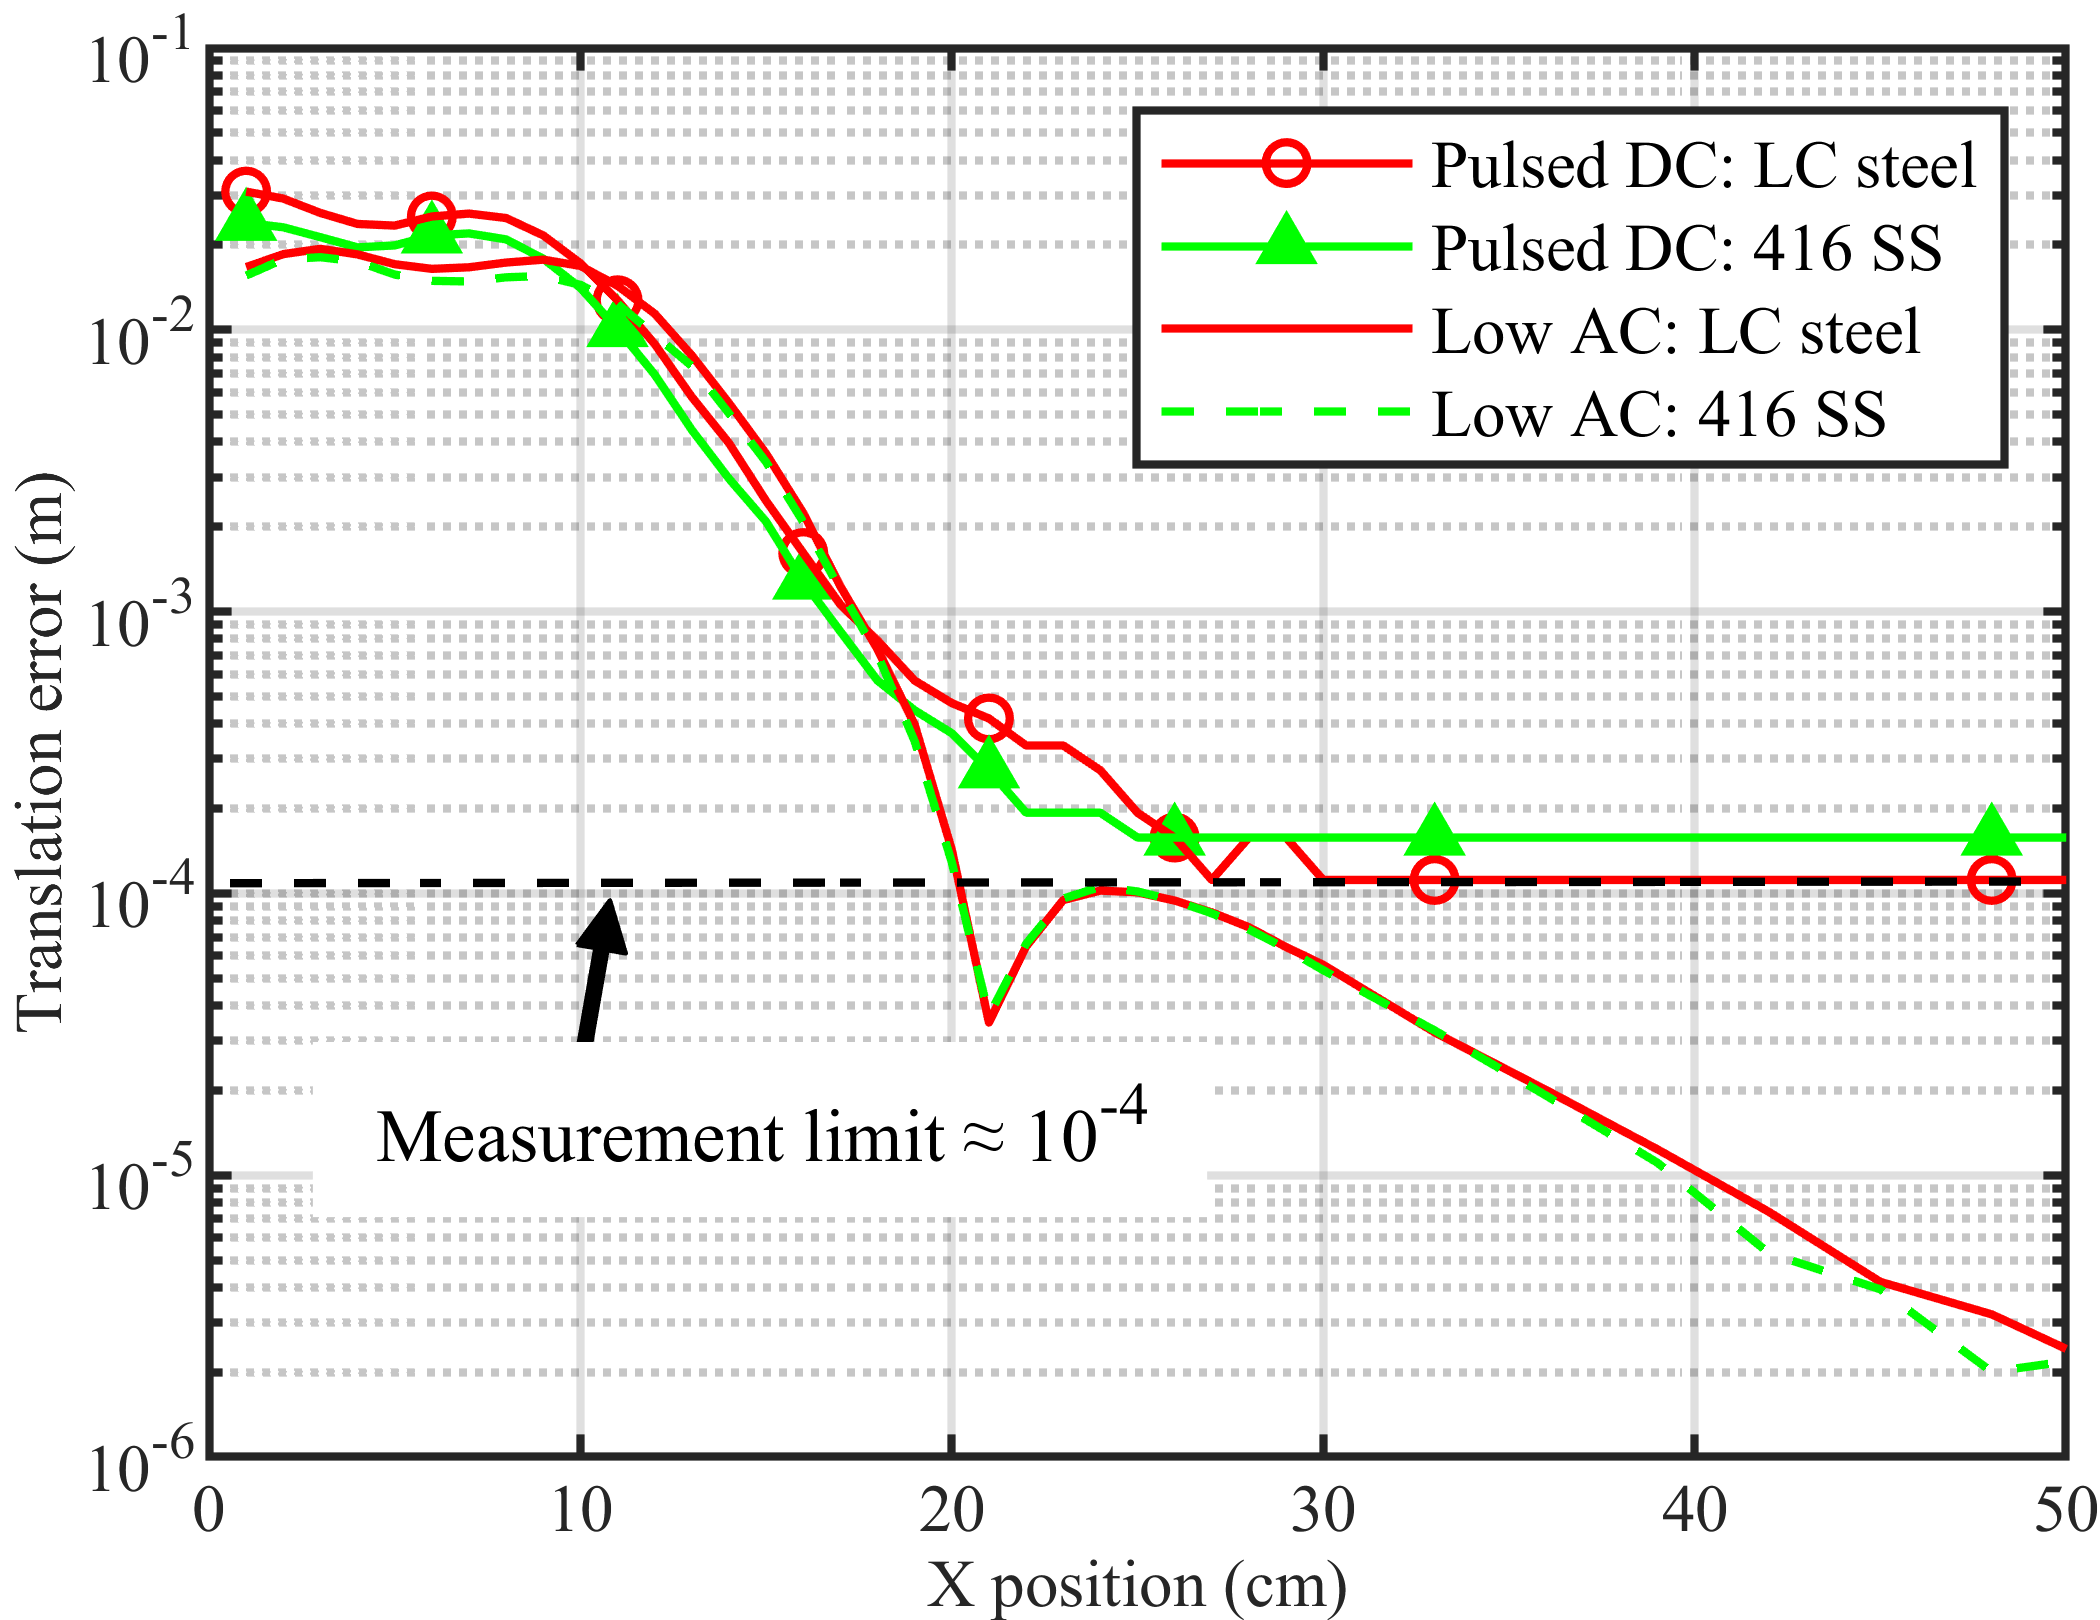
\includegraphics[width=\columnwidth]{chaic11.png}}
\caption{Translation error of tube samples during $x$ motion, comparing Low AC and Pulse modulation. For pulse modulation, only the ferromagnetic LC steel and 416 SS are visible above the trakSTAR detection limit. The errors are very similar between the two trackers, although the notch seems absent with trakSTAR.
(Modulations: Low AC and Pulse, Shape: Tube, Rotation: $0^\circ$)}
\label{xmoving_3DGuidance}
\end{figure} 

Fig. \ref{xmoving_3DGuidance} compares the $x$ motion response between Low AC and Pulse modulations. Because of trakSTAR's high measurement limit, we omit the non-ferromagnetic rod and tube samples which fall below its  $110\,\mu$m output quantization (see \S\ref{subsec:tested_emts}.) 

As predicted, the similar modulation frequencies of Pulse and Low AC modulation (\S\ref{subsec:tested_emts}) result in similar interference responses. The errors for the ferromagnetic rod and tube samples are almost identical across the modulations, and for the sheets the relative mismatch is still small (see supplement ~\ref{supplement:pulse_Low}). The similarity is particularly striking when we consider the seemingly quite different modulation and the entirely different hardware and software.

\subsection{Effect of Metal Shape} 
\label{sec:metal_shape}
\subsubsection{Rod vs. Tube}
\begin{figure}[tb]
\centerline{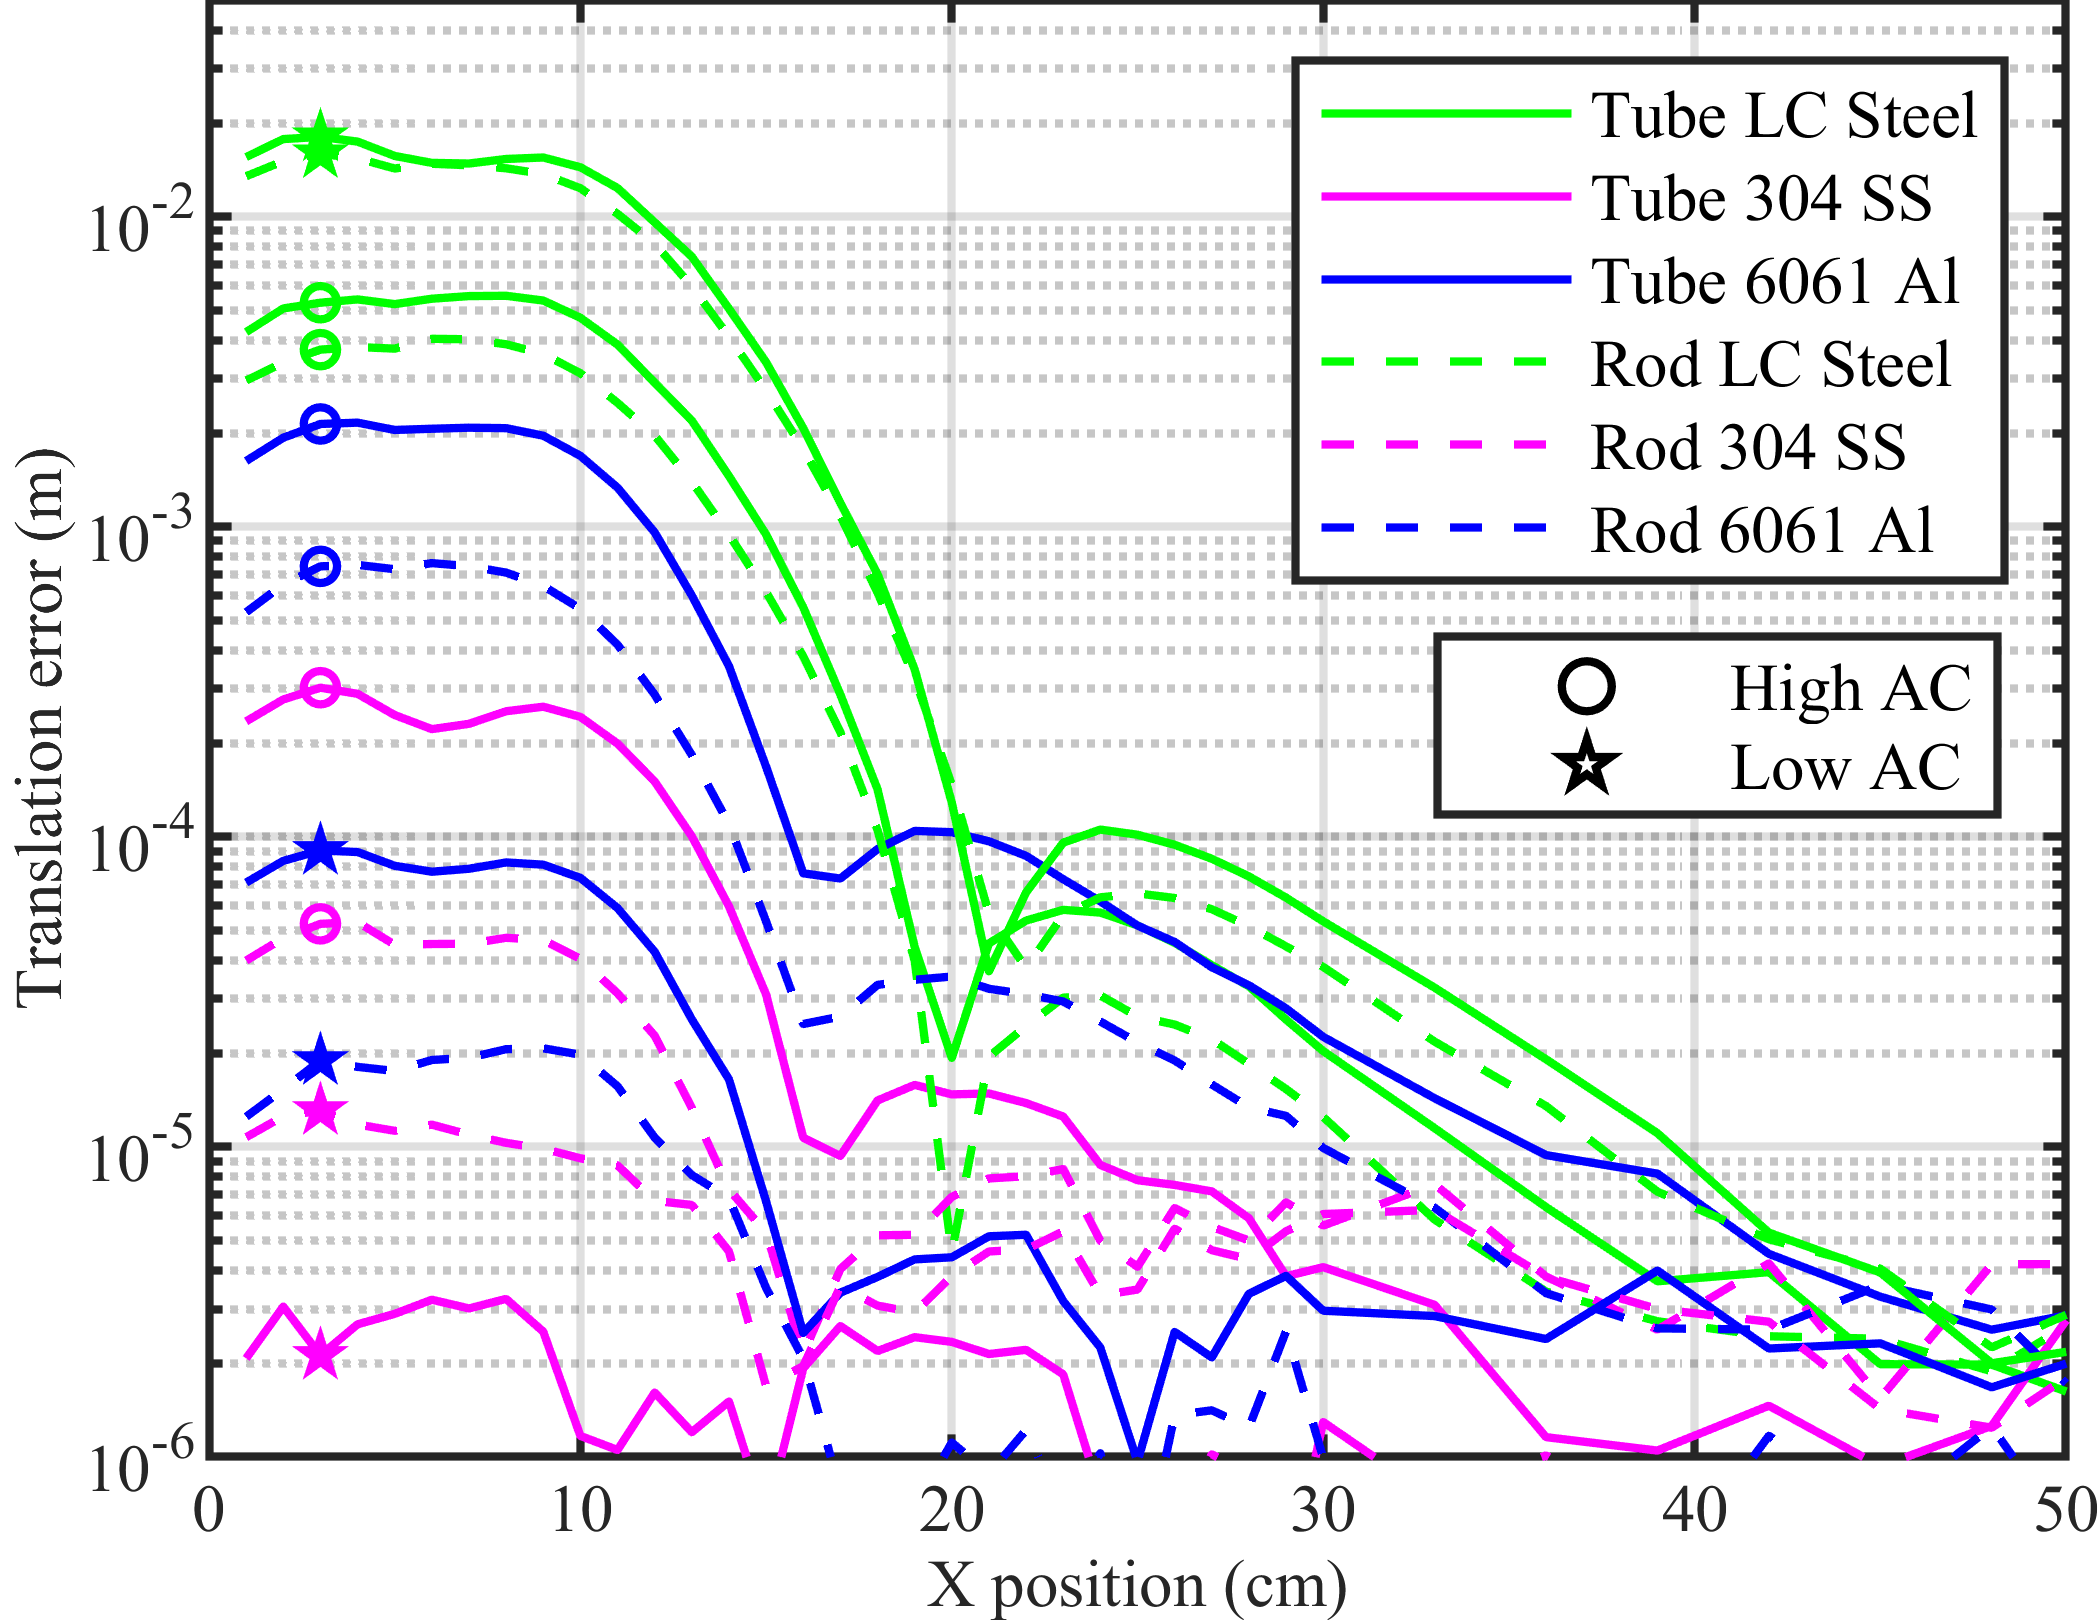
\includegraphics[width=\columnwidth]{chaic12.png}}
\caption{Translation error response to $x$ motion comparing rod and tube samples using High and Low AC modulations. For the ferromagnetic LC Steel the interference difference was small at High AC, disappearing at Low AC. With 304 SS at Low AC, the tube does create lower interference, dropping to the detection limit. For 6061 Al, the tube interference is larger at both modulations.
(Shapes: Tube and Rod, Modulations: High and Low AC, Rotation: $0^\circ$)}
\label{small_shape}
\end{figure}

From Fig. \ref{small_shape}, and returning to Fig. \ref{HighLow_compare}, we see that while the rods and tubes contained the same volume of metal and were the same length, there were material-dependent differences in the interference each created. Detailed discussion of the quantitative interaction of shape and modulation will be delayed to the discussion of Table \ref{Compare_HighLow_3DGuidance}, but note how the ferromagnetic LC Steel response is little affected by shape, especially at Low AC modulation where permeability dominates. In this case, the amount of metal is the main consideration. Also, for low conductivity 304 SS, the rod interference is clearly \textit{above} the measurement limit, while the tube is undetectable. 

Given the rod diameter of $7.9$ mm and tube wall thickness $1.3$ mm, we had thought we might see this reversal of tube and rod response for more materials (see \S\ref{subsec:metal_types}). For example, the skin depth for 6061 Al at 300\,Hz is $4.73\times10^{-3}$, exceeding the tube wall thickness $>3\times$. Yet the tube still creates much more interference than the rod.

\begin{figure}[H]
\centerline{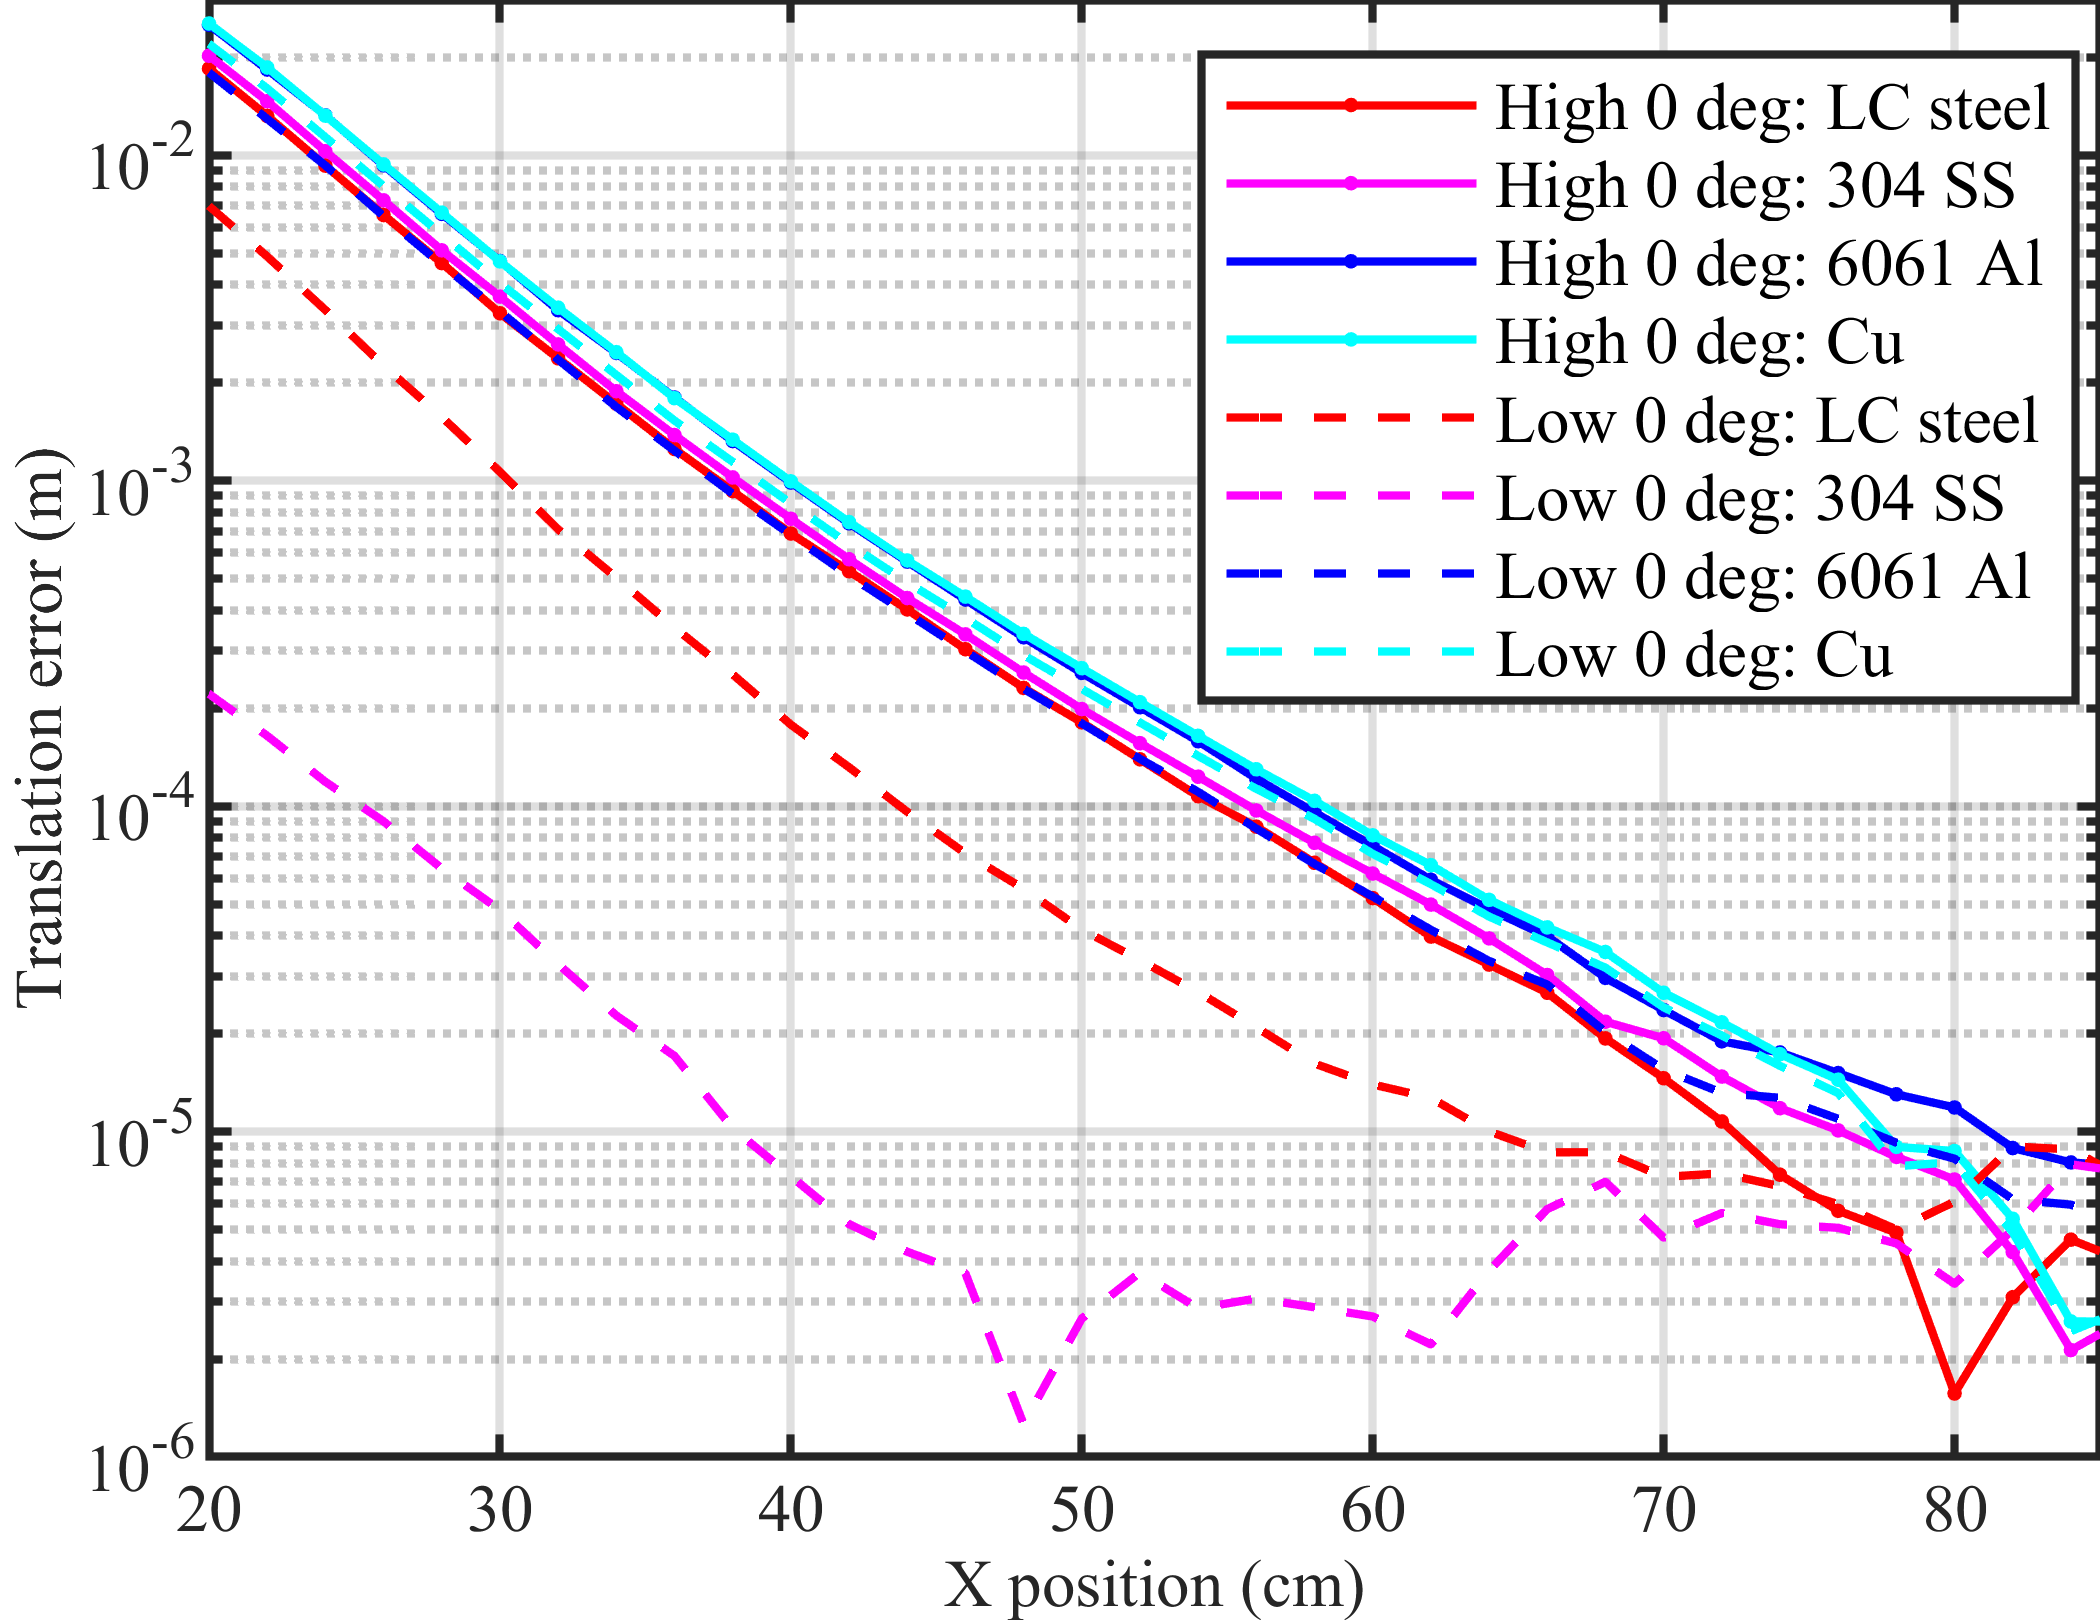
\includegraphics[width=\columnwidth]{chaic13.png}}
\caption{Response to $x$ motion for sheet samples and both High and Low AC modulations. Note that this motion started at $x = 20$ cm. The drop-off is remarkably uniform with very little difference between metals at High AC, while ferromagnetic LC Steel shows \textit{lower} interference at Low AC, contrary to its behavior with other shapes.
(Shape: Sheet, Modulations: High and Low AC, Rotation: $0^\circ$)}
\label{sheet_0deg}
\end{figure}

\subsubsection{Sheets}
\label{subsubsec:sheets_effect}

Our tests on the metal sheets gave the largest surprise we encountered during these experiments. Fig. \ref{sheet_0deg} shows the translation error response to $x$ motion. We did, unsurprisingly, confirm our hypothesis that the much larger and more massive sheet samples would create more interference at any given distance. This is not immediately obvious comparing Fig. \ref{sheet_0deg} to eg. Fig. \ref{small_shape} because sheet motion was started at $20$cm (Fig. \ref{location_example}) since the sheet did not fit between the source and sensor. For 6061 Al at High AC, the Fig. \ref{small_shape} tube has an error of $1\times 10^{-4}$ at $x=20$ cm, vs. $2\times 10^{-2}$ for the sheet in Fig. \ref{sheet_0deg}. Visually, comparing Fig. \ref{sheet_0deg} to Fig. \ref{small_shape}, the response curve appears quite different, with a very uniform drop-off lacking the \textit{flat} and \textit{notch} regions (labeled in Fig. \ref{hollow_high_xmoving}). Starting at $x=20$ cm certainly explains why we do not see the flat region, and the notch seen with rod and tube is likely a highly geometry-specific response of the pose solution algorithm, so this difference is not too surprising. 

The large surprise in Fig. \ref{sheet_0deg} is relatively low effect of metal type, and also that the ferromagnetic LC Steel shows \textit{lower} interference at Low AC modulation. These effects turn out to interact strongly with rotation, so we will delay further discussion.

\subsection{Effect of Metal Rotation}
\begin{figure}[H]
\centerline{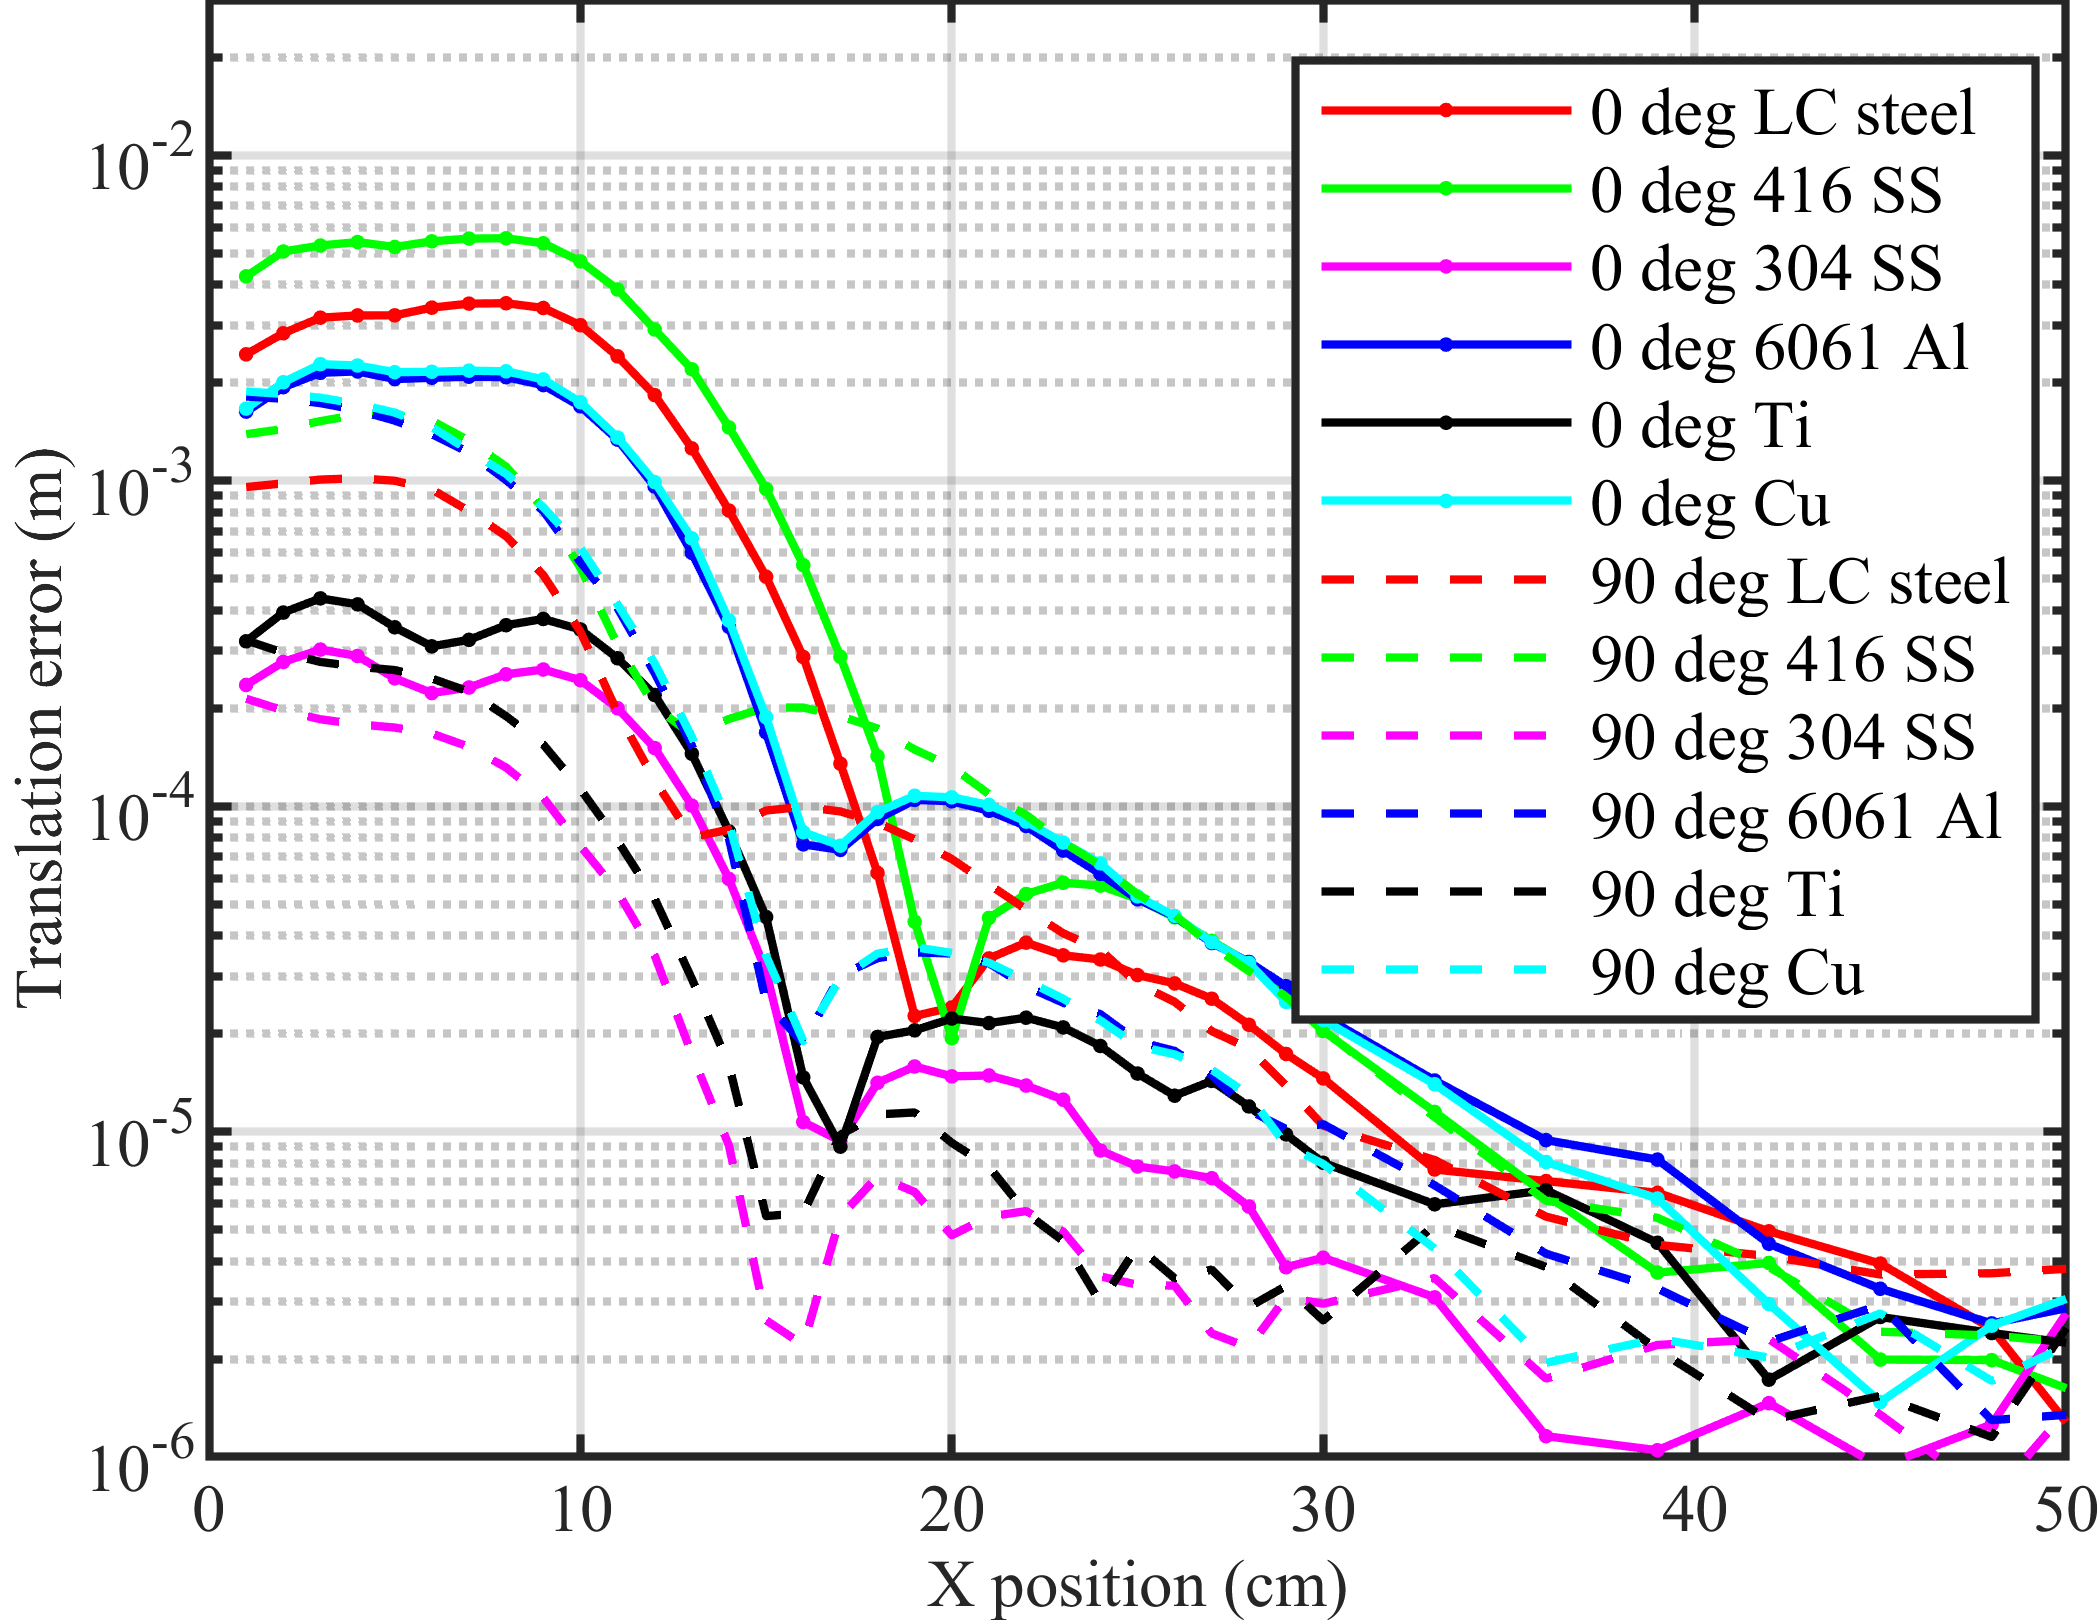
\includegraphics[width=\columnwidth]{chaic14.png}}
\caption{Translation error response to $x$ motion of tube samples at $0^\circ$ and $90^\circ$ rotations. Interference is generally lower at $90^\circ$ for $x < 25$ cm, with responses converging at larger distances, especially for ferromagnetic metals.
(Rotations: $0^\circ$ and $90^\circ$, Shape: Tube, Modulation: High AC)}
\label{90deg_high_tube}
\end{figure}

\subsubsection{Rod vs. Tube}
Fig. \ref{90deg_high_tube} compares the response to $x$ motion when tube samples are rotated. The interference decreases somewhat, especially at shorter ranges. This may be partly due to the metal center of mass being moved $5$ cm farther from the source-sensor axis. Excluding the notch location changes, the differences are fairly small, and seem to disappear for ferromagnetic samples at longer distances.

\subsubsection{Sheets}
Fig. \ref{sheet_90deg} shows the response to $x$ motion of sheets with $90^\circ$ rotation. Compare to Fig. \ref{sheet_0deg}, where we saw unexpected interactions with the metal type. Here the effect of metal is more similar to the hypothesized effects of conductivity and permeability (\S\ref{subsec:interference_mechanisms}), which we confirmed for the rod and tube shapes. As we saw with rod and tube rotation, the interference is lower at $90^\circ$. Here also, rotation moves the center of mass away from the source-sensor axis, now by $15$ cm. However, with sheets the reduction at $90^\circ$ is considerably larger than for rods and tubes, $\approx 25\times$. There are also significant differences in the interaction between metal type and modulation, such as the high/low ratio. These will be examined in more detail later in the Table \ref{Compare_HighLow_3DGuidance} discussion.

\begin{figure}[H]
\centerline{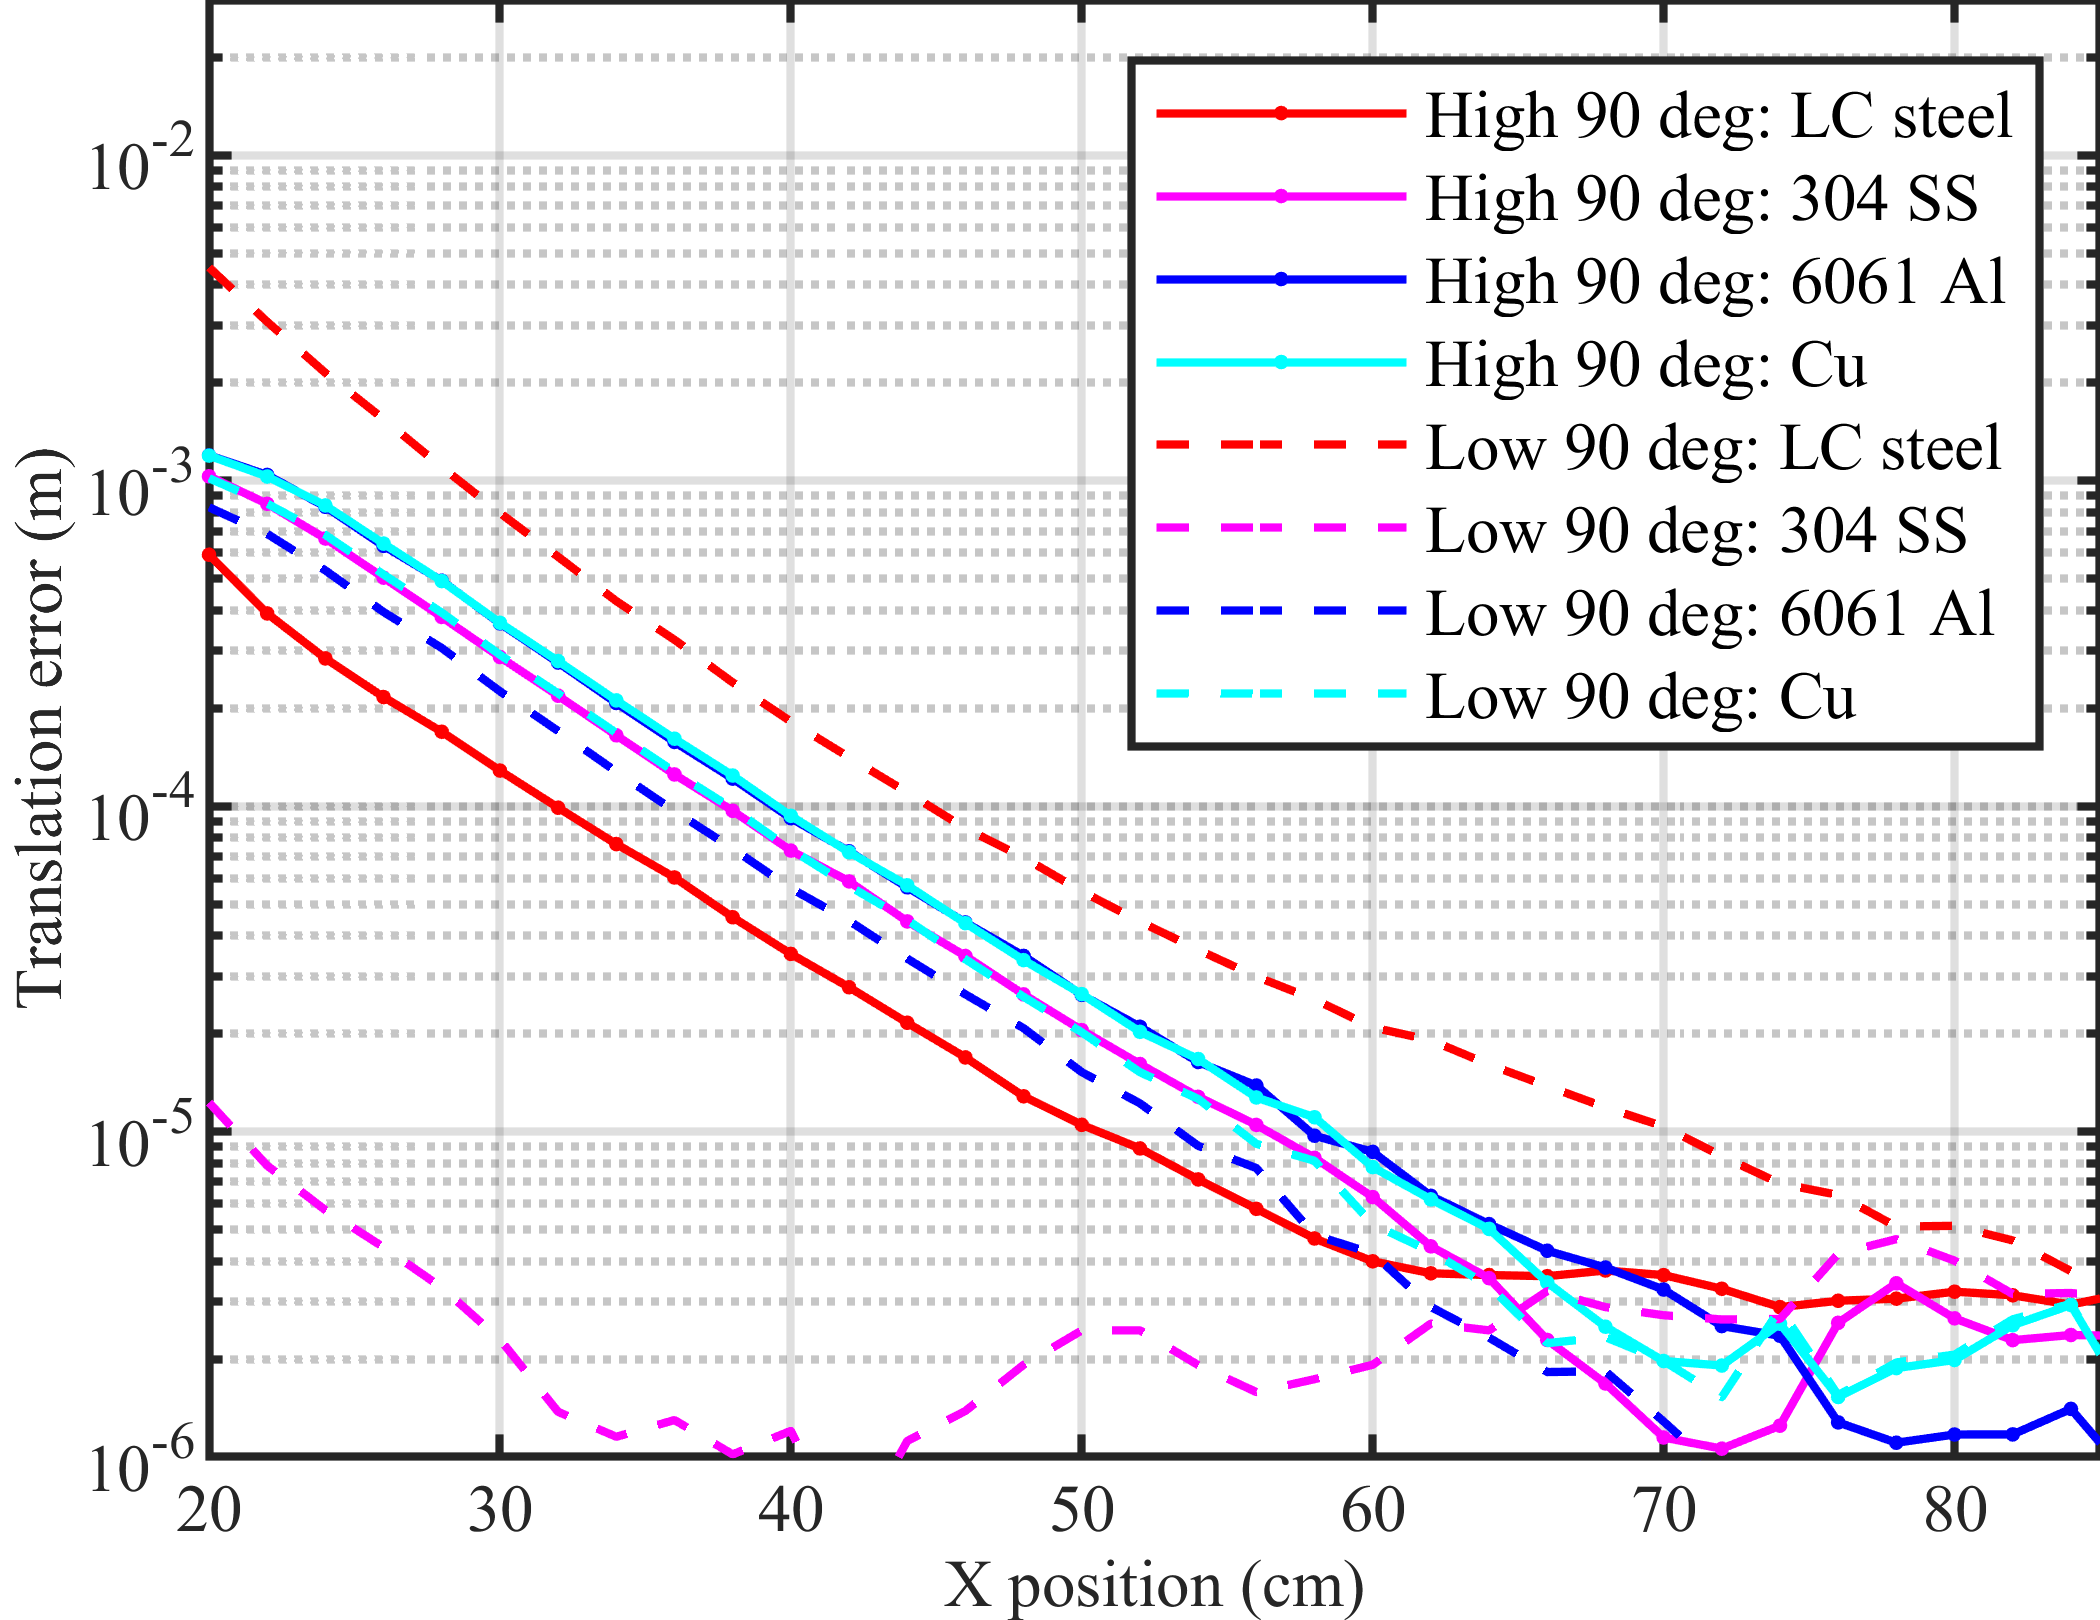
\includegraphics[width=\columnwidth]{chaic15.png}}
\caption{Translation error response to $x$ motion of sheet samples, $90^\circ$ rotation. Comparing to Fig. \ref{sheet_0deg} at $0^\circ$, the error is greatly reduced at $90^\circ$ and the interaction with metal type is more similar to what we have seen with rod and tube samples elsewhere.
(Rotation: $90^\circ$, Shape: Sheet, Modulations: High and Low AC)
}
\label{sheet_90deg}
\end{figure}


Why is the behavior so peculiar for sheets at $0^\circ$ orientation? Referring back to Fig. \ref{magnetic_field}, the magnetic field lines that would reach the sensor pass through the metal's thin edge, inducing small eddy currents, while field lines that wouldn't normally reach the sensor encounter the sheet's broad face, creating large eddy current loops that reflect these fields toward the sensor. Since these loops are very large, their high inductance (not conductivity) determines eddy current strength, explaining why all non-ferromagnetic metals show similar interference at High AC regardless of conductivity. For ferromagnetic LC Steel at $0^\circ$, the eddy current reflection dominates any permeability effects; its magnetic behavior is constrained by high demagnetization when interacting with the $y$-field, causing it to behave essentially as a moderate-conductivity metal with reduced interference at Low AC compared to High AC, unlike its behavior in other configurations.

\subsection{Power Law Fitting of Drop-off Behavior} \label{sec:Power Law}

\begin{figure}[tb]
\centerline{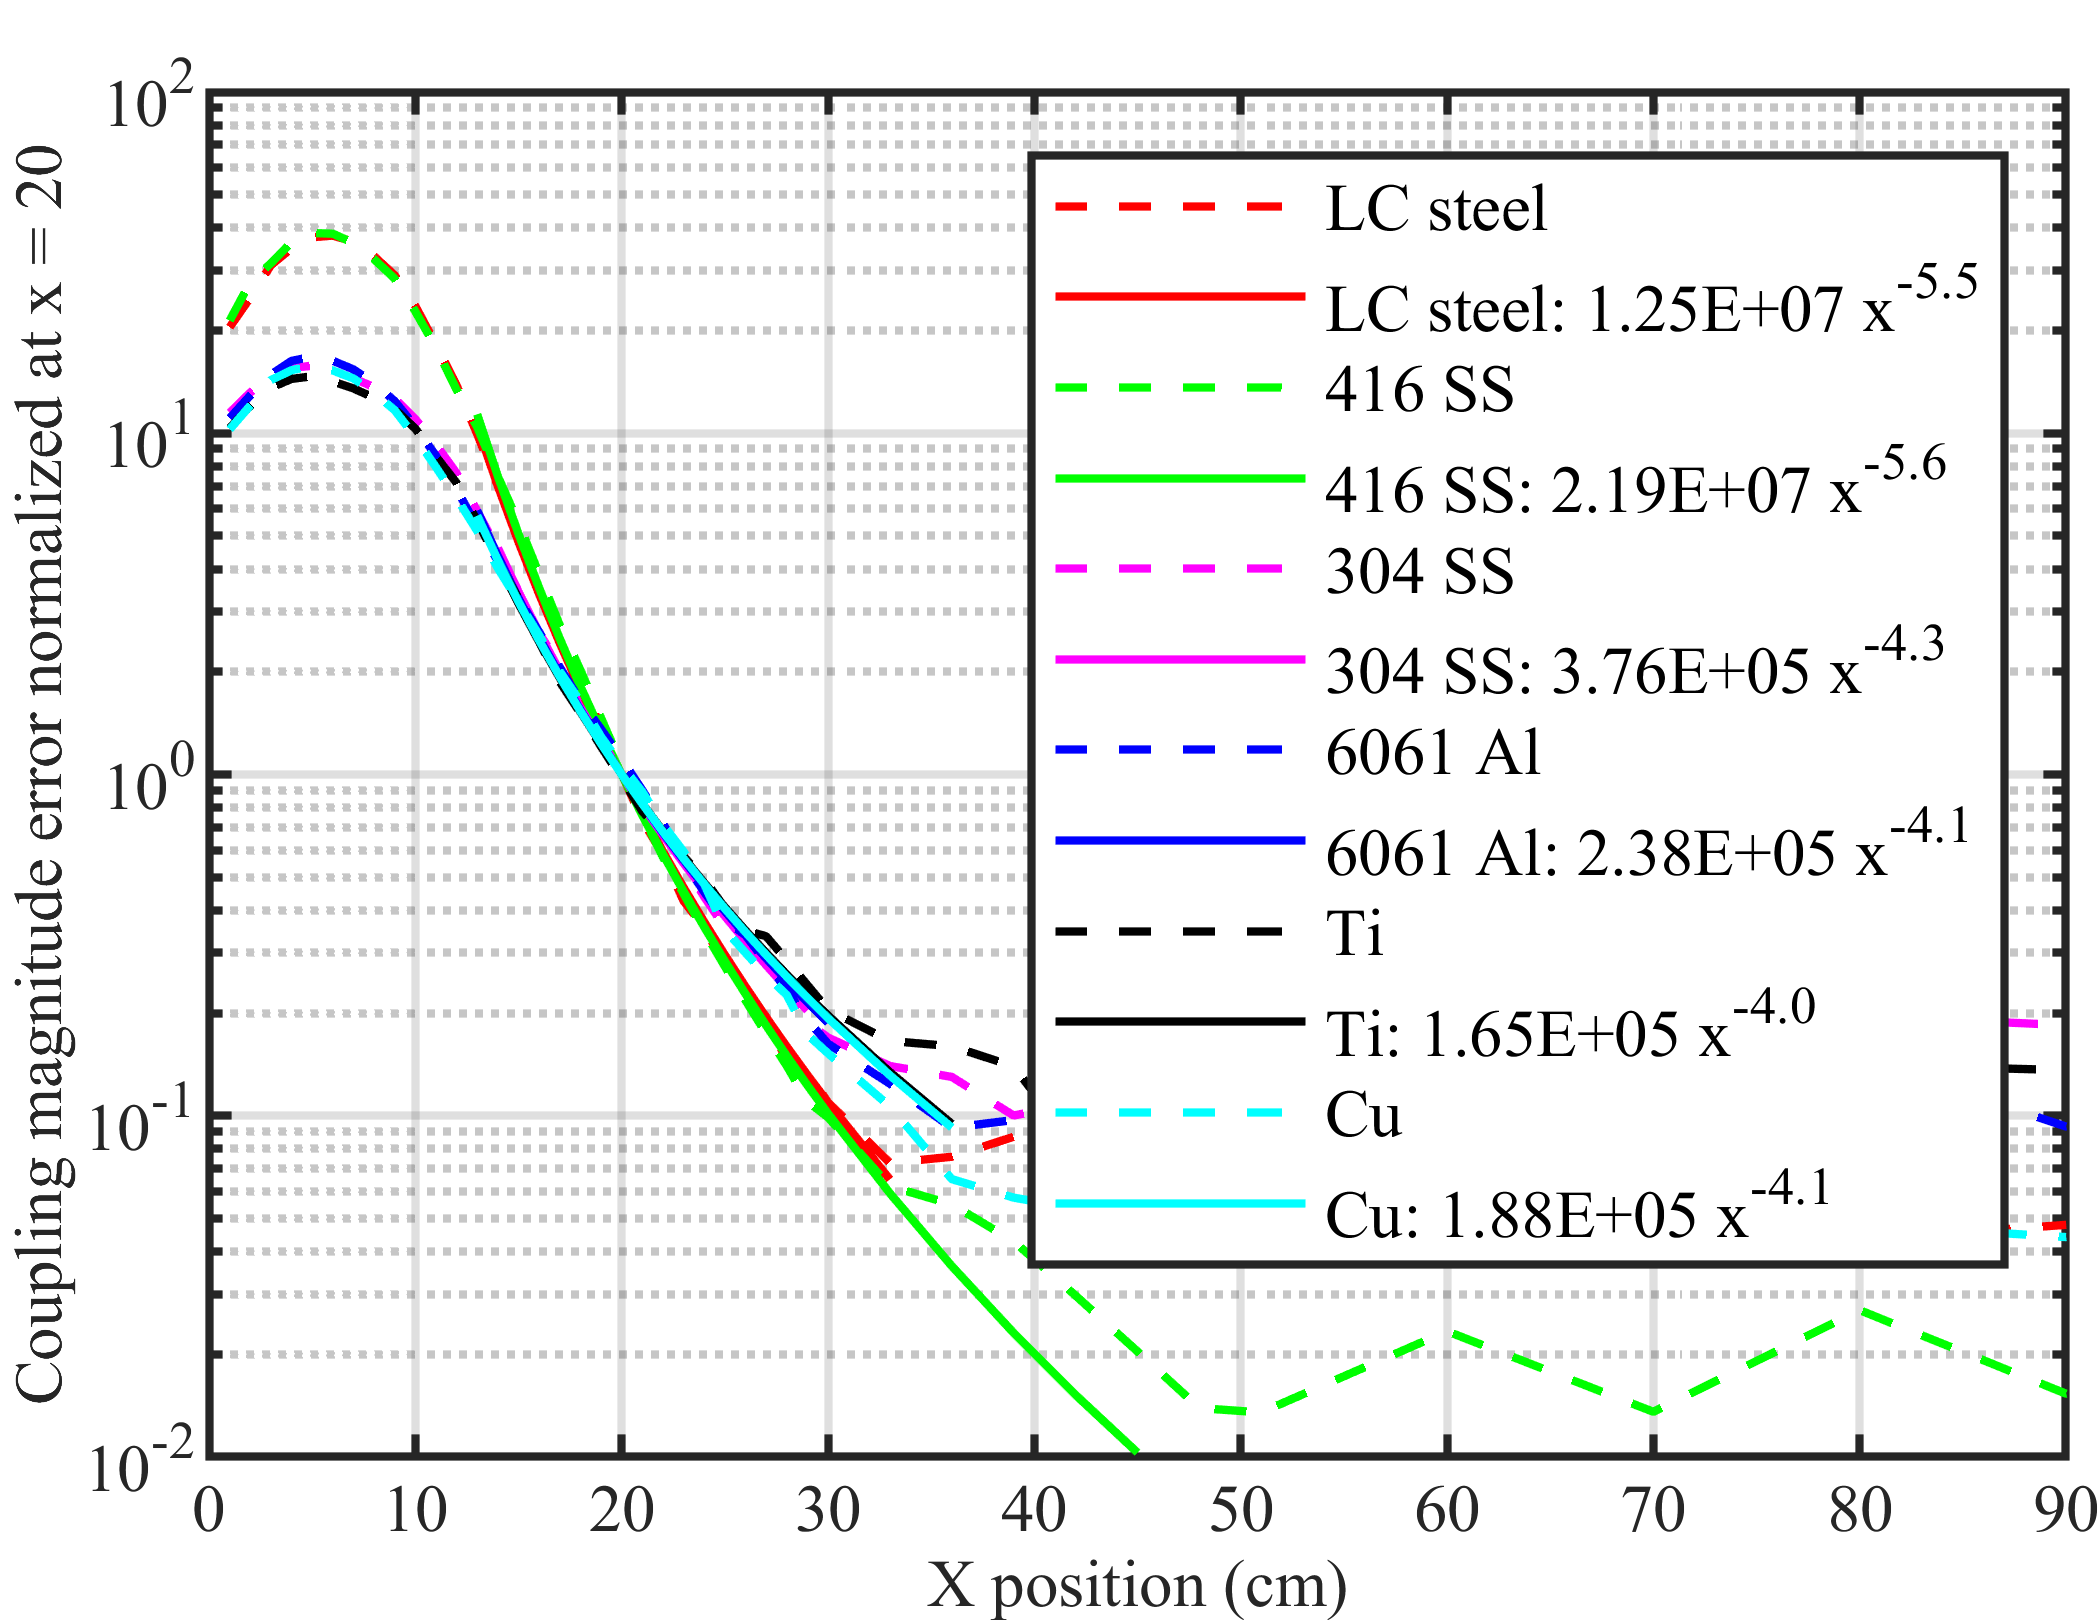
\includegraphics[width=\columnwidth]{chaic16.png}}
\caption{Power law fit of coupling error magnitude response to $x$ motion. The data for each sample is normalized so that the curve fit passes through (20, 1). There are two distinct response shapes for ferromagnetic and non-ferromagnetic metals, which is now much clearer than in the non-normalized Fig. \ref{xmoving_coupling}. For the ferromagnetic metals, the exponent magnitude is larger (steeper drop-off). 
(Shapes: Tube, Modulation: High AC, Rotation $0^\circ$)}
\label{coupling_fit}
\end{figure}

Beginning with Fig. \ref{hollow_high_xmoving} we observed that during $x$ motion the curve shapes were similar between metals even when the interference strength varied considerably at any given distance. There was also some difference in shape between the ferromagnetic and non-ferromagnetic metals. From theory \S\ref{nixon_model} we expect an $x^{-6}$ drop-off of interference with distance \eqref{eq:dropoff_power}, at least at far distance, so we have fitted our results to a power law response, Fig. \ref{coupling_fit}. These plots are normalized to equal error at $x=20$. The curves clearly now fall into ferromagnetic and non-ferromagnetic groups.

\begin{table}[!b]
\caption{Curve Fit Exponents (Modulation: High AC, Rotation: 0$^\circ$)}
\label{exponent}
\setlength{\tabcolsep}{3pt}
\centering
\begin{tabular}{|c|c|c|c|c|c|c|}
\hline
\parbox{45pt}{\centering {Metal Shape}} & 
\parbox{30pt}{\centering {LC steel}} & 
\parbox{30pt}{\centering {416 SS}} & 
\parbox{30pt}{\centering {304 SS}} &
\parbox{30pt}{\centering {6061 Al}} &
\parbox{20pt}{\centering {Ti}} &
\parbox{20pt}{\centering {Cu}} \\
\hline

Tube& $-5.5$& $-5.6$&$-4.3$&$-4.1$&$-4.0$&$-4.1$\\
Rod& $-5.7$& $-5.6$&$-3.1$&$-3.1$&$-3.2$&$-3.6$\\
Sheet& $-5.8$&$ $&$-5.9$&$-5.9$&$ $&$-5.9$\\

\hline
\end{tabular}
\end{table}

\begin{figure}[!b]
\centerline{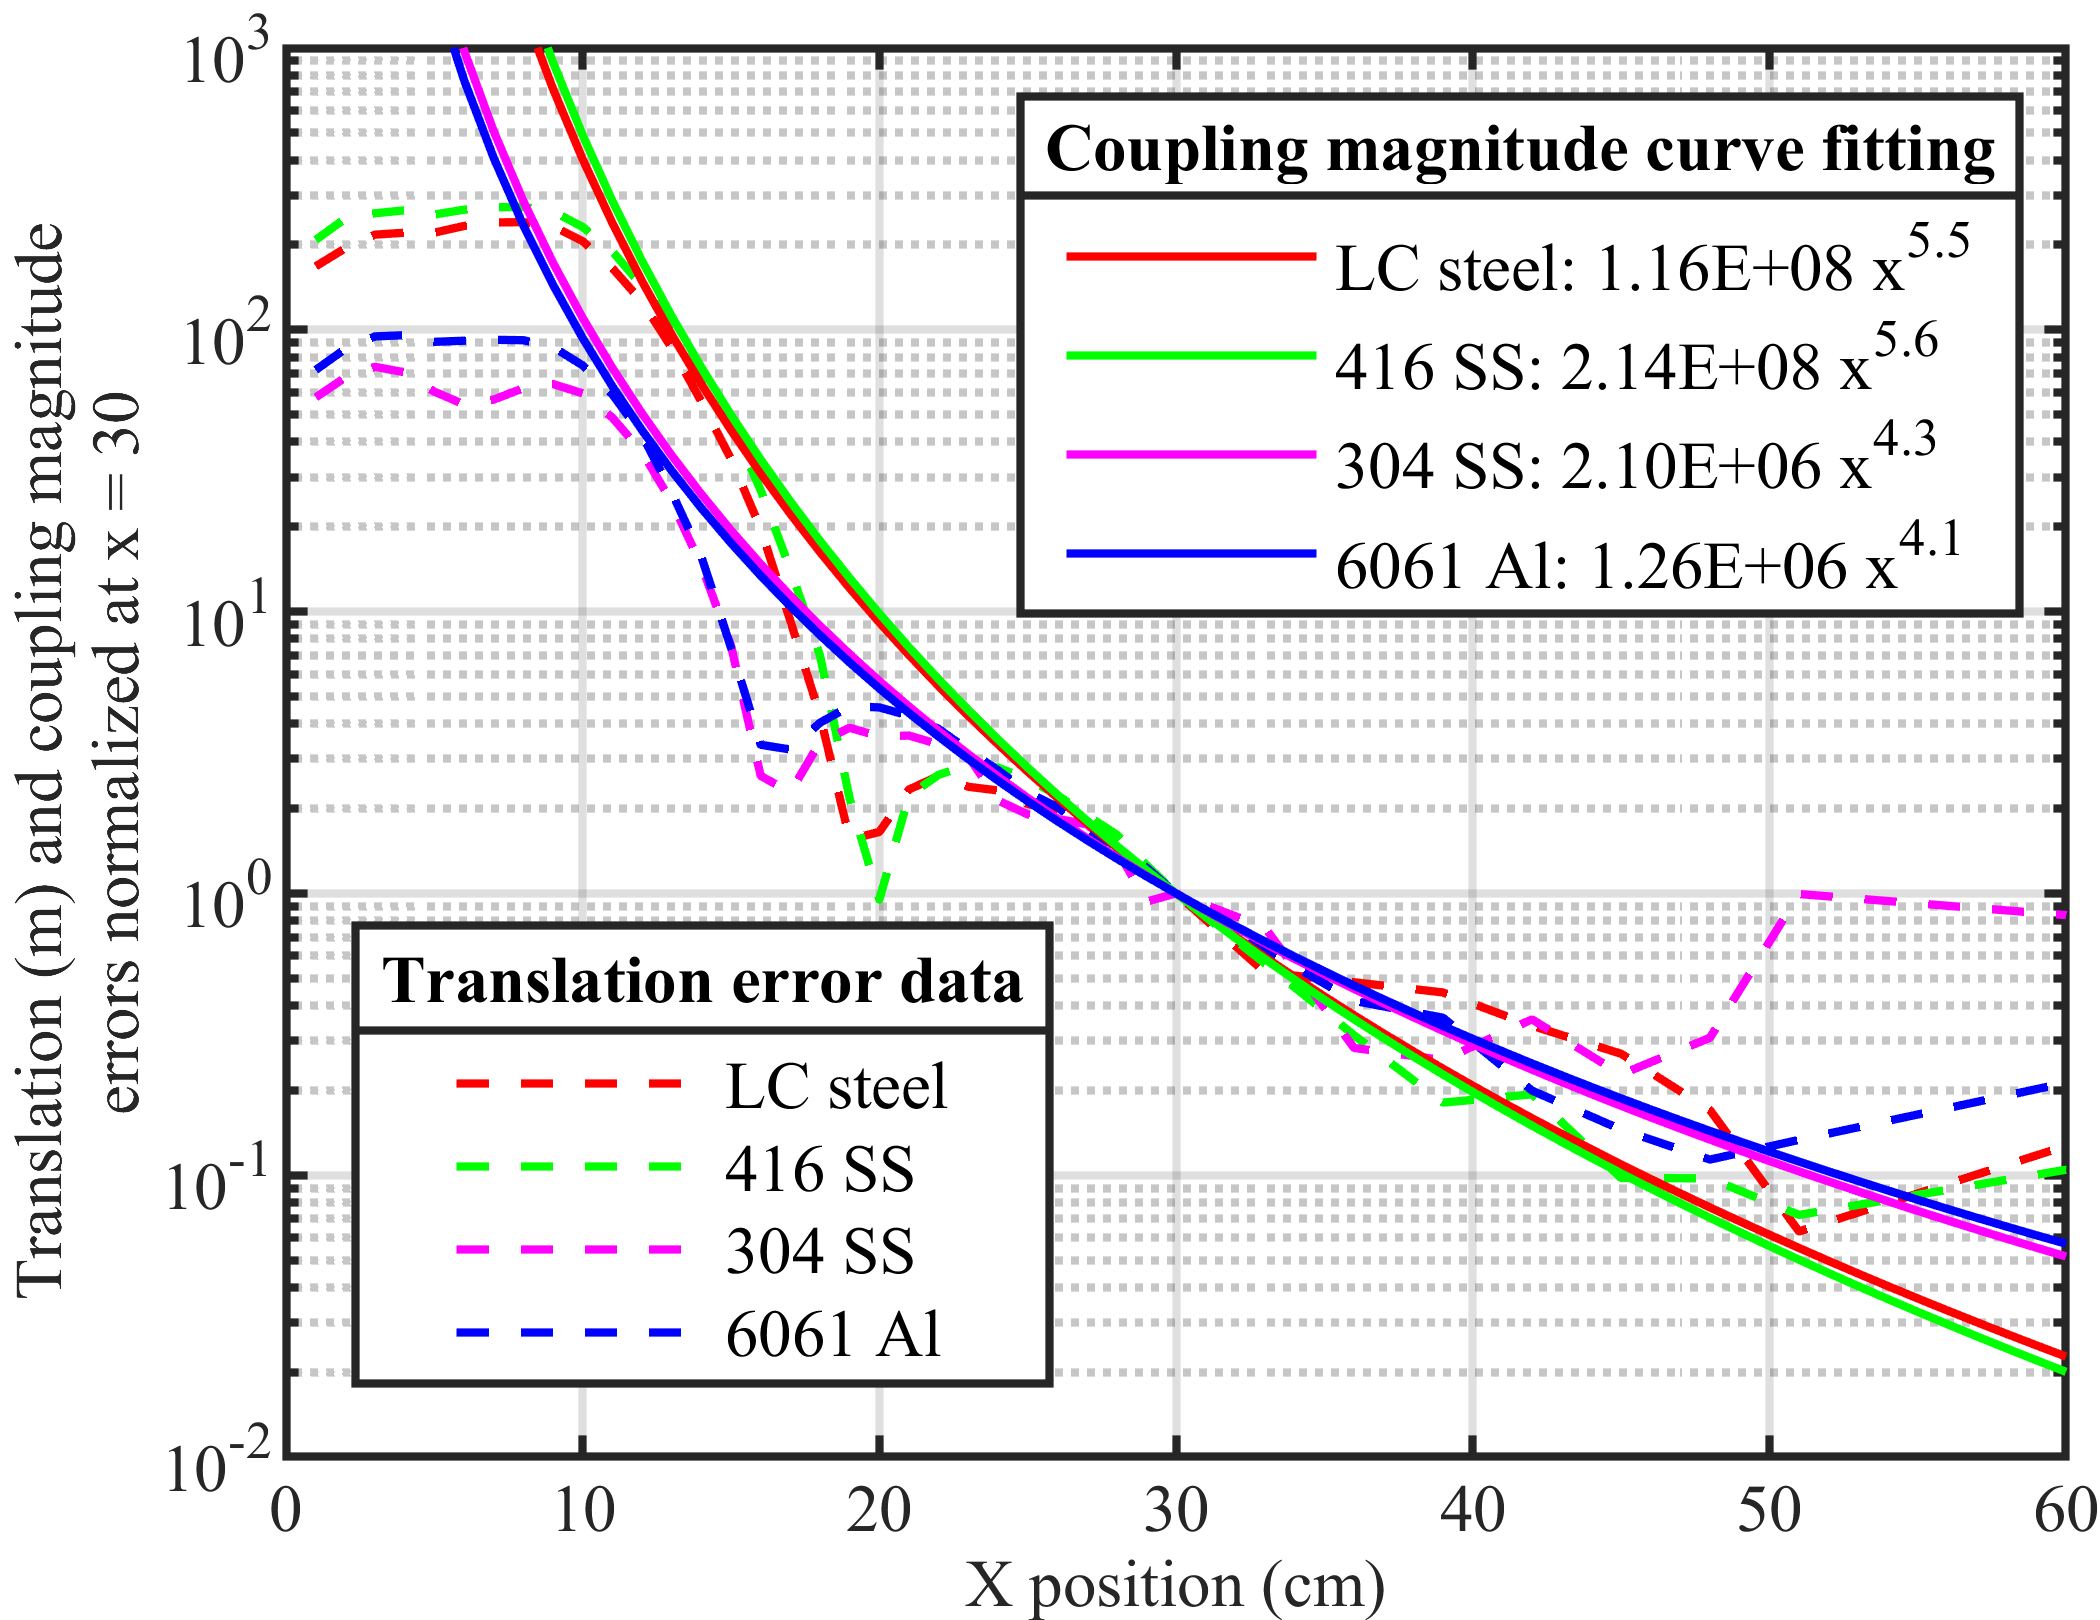
\includegraphics[width=\columnwidth]{chaic17.png}}
\caption{Translation error response to $x$ motion, with coupling error fits from Fig. \ref{coupling_fit} (a) superimposed by normalizing at $x = 30$ cm. Ignoring the notch in the translation error, the coupling error shape matches well over a wide range, and can be regarded as an upper bound.
(Shape: Tube, Modulation: High AC, Rotation $0^\circ$)}
\label{coup_trans_fit}
\end{figure}

Table \ref{exponent} shows the fitted exponents across all shapes and metals. All the sheets and all the ferromagnetic samples followed the -6 exponent dipole model fairly well, but non-ferromagnetic rod and tube samples showed significantly lower exponents between -3 and -4 (see supplement ~\ref{supplement:rod_fitting}, ~\ref{supplement:sheet_fitting}.) 

We fitted to coupling error because its curves lack the notch seen in the translation error. Fig. \ref{coup_trans_fit} superimposes the coupling error curve fits onto translation error data. Regarded as an upper bound, the power law fit from coupling matches the translation error well over nearly 3 orders of magnitude. 

\section{Summary}

\begin{table*}[!htbp]
\caption{Comparison of Modulation Effects vs. Metal and Shape (Translation Error)}
\label{Compare_HighLow_3DGuidance}
\setlength{\tabcolsep}{4pt}
\centering
\begin{tabular}{|l|c|c|c|c|c|c|}
\hline
\multicolumn{2}{|c|}{\parbox{75pt}{\centering {Metal Sample}}} & 
\parbox{60pt}{\centering {High AC}} & 
\parbox{60pt}{\centering {Low AC}} & 
\parbox{60pt}{\centering {High/Low Ratio}} & 
\parbox{60pt}{\centering {Pulse (trakSTAR)}} & 
\parbox{60pt}{\centering {Pulse/Low Ratio}} \\
\hline

LC steel 
&Tube& $3.01\times 10^{-3}$& $1.68\times 10^{-2}$& 0.18 &$1.72\times 10^{-2}$&1.02\\
$ $ &Rod& $2.32\times 10^{-3}$& $1.09\times 10^{-2}$ & 0.21 &$1.06\times 10^{-2}$&0.97\\
$ $ &Sheet& $2.60\times 10^{-2}$& $1.00\times 10^{-2}$ & 2.60 &$1.57\times 10^{-2}$&1.57\\
$ $ &Sheet ($90^\circ$)& $5.92\times 10^{-4}$& $4.53\times 10^{-3}$ & 0.13 &$4.78\times 10^{-3}$&1.06\\
\hline

416 SS 
&Tube& $4.72\times 10^{-3}$& $1.44\times 10^{-2}$& 0.33 &$1.41\times 10^{-2}$&0.98\\
$ $ &Rod& $3.13\times 10^{-3}$& $1.24\times 10^{-2}$ & 0.25 &$1.16\times 10^{-2}$&0.94\\
\hline

\multicolumn{4}{|r|}{Geometric mean:}& 0.32 &\multicolumn{2}{|c|}{$ $}\\
\hline

304 SS 
&Tube& $2.44\times 10^{-4}$& $1.17\times 10^{-6}$& 208.55 &$ $&$ $\\
$ $ &Rod& $4.04\times 10^{-5}$& $9.19\times 10^{-6}$ & 4.40$^{\dagger}$ &$ $& $ $\\
$ $ &Sheet& 
$2.48\times 10^{-2}$& $2.52\times 10^{-4}$ & 98.41 &
$ $&$ $\\
$ $ &Sheet ($90^\circ$)& 
$1.03\times 10^{-3}$& $1.23\times 10^{-5}$ & 83.74 &
$ $&$ $\\
\hline

6061 Al 
&Tube& $1.69\times 10^{-3}$& $7.37\times 10^{-5}$& 22.93 &$ $&$ $\\
$ $ &Rod& $5.44\times 10^{-4}$& $1.98\times 10^{-5}$ & 27.47 &$ $&$ $\\
$ $ &Sheet& $3.35\times 10^{-2}$& $2.43\times 10^{-2}$ & 1.38 &$1.87\times 10^{-2}$&$0.77$ \\
$ $ &Sheet ($90^\circ$)& $1.20\times 10^{-3}$& $8.29\times 10^{-4}$ & 1.45 &$7.57\times 10^{-4}$&$0.91$ \\
\hline

Ti 
&Tube& $3.49\times 10^{-4}$& $1.33\times 10^{-6}$& 262.41 &$ $&$ $\\
$ $ &Rod& $1.13\times 10^{-5}$& $2.56\times 10^{-6}$ & 4.41$^{\dagger}$ &$ $&$ $\\
\hline

Cu 
&Tube& $1.74\times 10^{-3}$& $2.75\times 10^{-4}$& 6.33 &$ $&$ $\\
$ $ &Rod& $6.04\times 10^{-4}$& $6.47\times 10^{-5}$ & 9.34 &$ $&$ $\\
$ $ &Sheet& $3.23\times 10^{-2}$& $2.83\times 10^{-2}$ & 1.14 &$2.37\times 10^{-2}$&$0.84$ \\
$ $ &Sheet ($90^\circ$)& $1.19\times 10^{-3}$& $1.02\times 10^{-3}$ & 1.17 &$1.25\times 10^{-3}$&$1.23$ \\
\hline

\multicolumn{4}{|r|}{Geometric mean:}& 11.67 & \multicolumn{2}{|c|}{\centering {$ $}}\\
\hline
\end{tabular}

\vspace{0.5em}
\footnotesize{Note: Translation errors are measured at $x = 10$ cm for rod/tube samples and $x = 18$ cm for sheet samples, so the error magnitudes for sheets are not directly comparable to rod and tube. For the High/Low Ratio, larger values indicate greater interference reduction at low frequencies. This ratio varies greatly with metal type and shape. The Pulse/Low Ratio compares Pulse modulation to Low AC, where values are all near $1$, indicating very similar behavior.

"$\dagger$" marks ratios that are likely underestimated because the interference at High AC is already barely measurable.}
\end{table*}

Table \ref{Compare_HighLow_3DGuidance} provides a quantitative summary of metal, shape, modulation and rotation effects at a fixed distance.

\textbf{Effect of Modulation.} The $\mathrm{high}/\mathrm{low}$ ratio varies widely, but using the robust geometric mean we can generalize that low frequency modulations (300\,Hz and Pulse) reduce typical interference for non-ferromagnetic metals by 12$\times$ compared to High AC (10\,kHz). Conversely, these same low frequencies increase typical interference for ferromagnetic metals by 3$\times$. The similar frequency content of Low AC and Pulse modulations results in nearly identical interference despite using different tracker hardware and signal processing. 

\begin{table}[!htbp]
\caption{Eddy Current Field Distortion Ratios for Different Metals (loop model)}
\label{tab:distortion_ratios}
\setlength{\tabcolsep}{4pt}
\centering
\begin{tabular}{|l|c|c|c|}
\hline
Material & 300 Hz & 10\,kHz & Ratio (10\,kHz / 300 Hz) \\ 
\hline
Copper & $2.13e-04$ & $0.001158$ & $5.44$ \\
Aluminum & $1.28e-04$ & $0.001134$ & $8.84$ \\
Stainless & $5.05e-06$ & $1.67e-04$ & $32.97$ \\
\hline
\end{tabular}
\end{table}

Table \ref{tab:distortion_ratios} shows the high/low field distortion ratios predicted by the \S\ref{subsubsec:eddy_current_model} eddy current loop model for different metals. These numbers do capture the trend for reduced high/low ratios in high conductivity metals, but, surprisingly, the high/low ratios for the low conductivity metals sometimes greatly exceed $10\,\mathrm{kHz}/300\,\mathrm{Hz} = 33$, which the loop model cannot explain. Note that the rod ratios marked with "$\dagger$" are likely underestimated because the interference at High AC is already barely measurable. 

\textbf{Effect of Metal Type.}
Interference generally decreases in this order: ferromagnetic metals, high-conductivity non-ferromagnetic metals, and low-conductivity non-ferromagnetic metals, however this varies with metal shape and orientation, with sheets at $0^\circ$ rotation being a strong exception. Ferromagnetic materials experience both eddy current and permeability distortions, but the permeability effect typically dominates. Eddy current strength correlates with conductivity for non-ferromagnetic metals, but (especially with High AC modulation) the difference between Cu and 6061 Al can largely disappear. 

\textbf{Effect of Metal Shape and Size.}
Compared to rods and tubes, the large sheets create much more interference, but Table \ref{Compare_HighLow_3DGuidance} obscures this because the sheets are placed at a longer distance, see \S\ref{subsubsec:sheets_effect}. Surprisingly, even when skin depth significantly exceeds tube wall thickness, the tube typically generates more interference than the solid rod of the same metal volume. Sheet samples show complex behavior that varies with orientation and material type, deviating from expected patterns due effects not captured by simple models, e.g. both conductivity \textit{and} permeability have minimal effect for sheets at $0^\circ$. 

\textbf{Effect of Metal Rotation.}
Samples oriented at $90^{\circ}$ generally show lower interference due to changes in both demagnetization and current loop patterns. The interaction between rotation, shape, and metal type create unexpected behavior, particularly with sheet samples, where rotation has a large $\approx 25\times$ effect and also changes which metals show the greatest interference. 

\section{Conclusion}
This study provides insights into metallic interference with electromagnetic trackers across multiple variables. For EMT users operating in environments where metallic objects cannot be avoided, we offer several practical recommendations. \textbf{First}, minimize the presence of metallic materials in the tracking workspace, particularly large objects like sheets. \textbf{Second}, when metals are necessary, select non-ferromagnetic materials with lower conductivity like Ti or 304 SS rather than ferromagnetic metals like LC steel and 416 SS. \textbf{Third}, position metallic objects as far from the source-sensor axis as possible, as interference decreases with distance following approximately an inverse fourth to sixth power relationship. \textbf{Fourth}, avoid orienting of metal objects parallel to the source-sensor axis.

The choice of tracker modulation technology significantly affects metal compatibility. For environments with predominantly non-ferromagnetic metals, low-frequency modulations (either Low AC or Pulse DC) dramatically reduce interference. However, when ferromagnetic metals cannot be avoided, high-frequency modulation may be preferable. ILEMT's dual-frequency capability offers a promising approach, potentially allowing adaptive selection of the optimal modulation based on the specific interference environment.

For EMT developers, our findings highlight the limitations of simple dipole models for metal interference, particularly with larger metal objects or when positioned close to the source or sensor. The drop-off in interference with distance varies significantly based on metal type, shape, and orientation. The complex relationships between pose error and field deviation suggest that sophisticated interference compensation algorithms may need to consider the specific characteristics of the pose solution rather than simply modeling field changes.

Future work could explore using modulation phase information to detect and classify metal interference, potentially allowing adaptive algorithms to select the optimal frequency band or to combine measurements for improved accuracy. The ILEMT approach of simultaneous multi-frequency measurement offers unique opportunities to develop real-time interference detection and compensation techniques that could significantly expand the viable applications of electromagnetic tracking in challenging environments.

\section*{Acknowledgment}
The authors sincerely appreciate Boyle C. Cheng for the valuable help in reviewing and improving the manuscript. In addition, generative AI was used in this manuscript to improve clarity and grammar.

\bibliographystyle{ieeetr}
\bibliography{references}

\end{document}